\documentclass[10pt,journal,compsoc]{IEEEtran}
\usepackage{graphicx}
\usepackage{amsfonts}
\usepackage{color}
\usepackage[pdftex]{hyperref}
\usepackage{epstopdf}
\usepackage[ruled,vlined]{algorithm2e}
\usepackage{subcaption}
\usepackage{amsmath}
\usepackage{amssymb}
\usepackage{hyperref}
\usepackage{mathrsfs}
\usepackage{latexsym}
\usepackage{multirow}
% \usepackage[caption=false]{subfig}
\usepackage[export]{adjustbox}

\ifCLASSOPTIONcompsoc
  \usepackage[nocompress]{cite}
\else
  \usepackage{cite}
\fi


% new command section, Thanks for JMO for the suggestion to keep the document clean and unified.


% The newcommand file to define the variables

\usepackage{xspace}

\newcommand{\mbf}{\mathbf}
%\DeclareMathOperator*{\argmin}{arg\,min}

\newcommand{\mypartitle}[2][2]{\vspace*{-#1 ex}~\\{\noindent {\bf #2}}}
\newcommand{\mypartitletwo}[1]{\vspace*{-1.5ex}~\\{\noindent \underline{\bf #1}}}

\newcommand{\mycomline}[1]{~\\[0mm]{JMO comment: {\color{blue} #1}}~\\}

\newcommand{\dwucomline}[1]{~\\[0mm]{DWU comment: {\color{red} #1}}~\\}

%%%%%%%%%%%%%%%%%%%%%%%%%%%%%%%%%%%%%%%%%%%%%%%%%
%HMM
%%%%%%%%%%%%%%%%%%%%%%%%%%%%%%%%%%%%%%%%%%%%%%%%%
% random variable
\newcommand{\observation}{\ensuremath{X}\xspace}
\newcommand{\observationSK}{\ensuremath{\observation^{s}}\xspace}
\newcommand{\observationRGBD}{\ensuremath{\observation^{s}}\xspace}
\newcommand{\randomvariable}{$\observation_t$}

% hidden variable
\newcommand{\hiddenstate}{\ensuremath{H}\xspace}
\newcommand{\hiddenstatenode}{\ensuremath{h}\xspace}
\newcommand{\hiddenvariable}{$\hiddenstate_t$}

% finite set
\newcommand{\finiteset}{\ensuremath{\mathcal{H}}\xspace}
% number of hidden states
\newcommand{\numberhiddenstate}{\ensuremath{N_{\finiteset}}\xspace}

% transition matrix
\newcommand{\transitionmatrix}{$p(\hiddenstate_t | \hiddenstate_{t-1})$}

% emission probability
\newcommand{\emissionprob}{\ensuremath{p(\observation_t | \hiddenstate_t)}\xspace}

\newcommand{\emissionprobSK}{\ensuremath{p(X_t^S | H_t)}\xspace}

\newcommand{\emissionprobRGBD}{\ensuremath{p(X_t^R | H_t)}\xspace}
% general input for hmm
\newcommand{\inputhmm}{$x_i$}

% general frame label for hmm
\newcommand{\framelabelhmm}{$y_i$}

% ergodic state
\newcommand{\ergodicstate}{$\mathcal{ES}$}
%%%%%%%%%%%%%%%%%%%%%%%%%%%%%%%%%%%%%%%%%%%%%%%%
% HMM numbers

% number of states associated to an individual gesture
\newcommand{\nsig}{$N_{\mathcal{H}_a}$}
% total number of states
\newcommand{\tns}{$N_{\mathcal{H}}$}

%%%%%%%%%%%%%%%%%%%%%%%%%%%%%%%%%%%%%%%%%%%%%%%%%
%  input
%%%%%%%%%%%%%%%%%%%%%%%%%%%%%%%%%%%%%%%%%%%%%%%%%
% skeleton input
\newcommand{\randomvariableSK}{$\observation_t^s$}
% skeleton high level features
\newcommand{\highSK}{\ensuremath{V^s}\xspace}

% RGBD input
\newcommand{\randomvariableRGBD}{$\observation_t^r$}
%RGBD high level features
\newcommand{\highRGBD}{\ensuremath{V^r}\xspace}

% gesture a
\newcommand{\gesturea}{$\textbf{\emph{a}}$}

% number of joints used
\newcommand{\numberofjoints}{$N_j$}

% skeleton features at time t
\newcommand{\skfeaturet}{$x_t^s$}

% skeleton features
\newcommand{\skfeature}{$f_t$}

% number of hidden state
\newcommand{\numberhiddenstates}{\ensuremath{N_\mathcal{H}}}


% Result section
\newcommand{\jaccardindex}{\ensuremath{J\hspace*{-0.1em}I}\xspace}
\newcommand{\eventaccuracy}{\mbox{\emph{Recognized}}\xspace}
\newcommand{\eventconfused}{\mbox{\emph{Confused}}\xspace}
\newcommand{\eventmissed}{\mbox{\emph{Missed}}\xspace}









\begin{document}

\title{Deep Dynamic Neural Networks for Multimodal Gesture
Segmentation and Recognition}

\author{Di~Wu,
        Lionel~Pigou,
        Pieter-Jan Kindermans,
        Nam~Le,
        Ling~Shao,
        Joni Dambre,
        and~Jean-Marc Odobez
%\IEEEcompsocitemizethanks{\IEEEcompsocthanksitem M. Shell is with the Department
%of Electrical and Computer Engineering, Georgia Institute of Technology, Atlanta,
%GA, 30332.\protect\\
%% note need leading \protect in front of \\ to get a newline within \thanks as
%% \\ is fragile and will error, could use \hfil\break instead.
%E-mail: see http://www.michaelshell.org/contact.html
%\IEEEcompsocthanksitem J. Doe and J. Doe are with Anonymous University.}% <-this % stops an unwanted space
%\thanks{Manuscript received April 19, 2005; revised September 17, 2014.}
}


% The paper headers
\markboth{IEEE TRANSACTIONS ON PATTERN ANALYSIS AND MACHINE INTELLIGENCE, December~2014}%
{Shell \MakeLowercase{\textit{et al.}}: Bare Demo of IEEEtran.cls for Computer Society Journals}


\IEEEtitleabstractindextext{%

\begin{abstract}
This paper describes a novel method called Deep Dynamic Neural Networks \emph{(DDNN)} for  multimodal gesture recognition.
%
More precisely, a semi-supervised hierarchical dynamic framework based on a Hidden Markov Model (HMM) 
is proposed for simultaneous gesture segmentation and recognition where skeleton joint information, 
depth and RGB images are the multimodal input observations.
%
Unlike most traditional approaches which rely on the construction of complex handcrafted features, 
our approach learns high-level spatio-temporal representations using  deep neural networks suited to the input modality: 
a Gaussian-Bernouilli Deep Belief Network (\DBN)  to handle skeletal dynamics, 
and a 3D Convolutional Neural Network (\ThreeDCNN) to manage and fuse batches of  depth and RGB images.
%
This is achieved through the modeling and learning of the  emission probabilities of the HMM required to infer the gesture sequence.
%The framework can be easily extended by including an ergodic state to segment and recognize video sequences by a frame-to-frame mechanism, making online segmentation and recognition possible.
This purely data driven approach achieves a Jaccard index score of \textbf{\emph{0.81}} in the ChaLearn LAP gesture spotting challenge. 
The performance is on par with a variety of state-of-the-art hand-tuned feature-based approaches and other learning-based methods, therefore opening the door on using deep learning techniques to further explore multimodal time series.
\end{abstract}


\endinput








%% PREVIOUS VERSION
\begin{abstract}
This paper describes a novel method called deep Dynamic Neural Networks \emph{(DDNN)} for  multimodal gesture recognition.
A semi-supervised hierarchical dynamic framework is proposed for simultaneous gesture segmentation and recognition taking skeleton, depth and RGB images as input observations.
Unlike the traditional construction of complex handcrafted features, all inputs are learnt by deep neural networks: the skeletal module is modeled by Deep Belief Networks \emph{(DBN)}; the depth and RGB module are modeled by 3D Convolutional Neural Networks \emph{(3DCNN)} to extract high-level spatio-temporal features.
The learned representations are then used for estimating emission probabilities of the Hidden Markov Models to infer a gesture sequence.
The framework can be easily extended by including an ergodic state to segment and recognize video sequences by a frame-to-frame mechanism, making online segmentation and recognition possible.
This purely data driven approach achieves a score of \textbf{\emph{0.81}} in the ChaLearn LAP gesture spotting challenge. The performance is on par with a variety of the state-of-the-art hand-tuned feature approaches and other learning-based methods, opening the doors for using deep learning techniques to explore multimodal time series.
\end{abstract}


% Note that keywords are not normally used for peerreview papers.
\begin{IEEEkeywords}
Deep learning, convolutional neural networks, deep belief networks, hidden Markov models,
gesture recognition.
\end{IEEEkeywords}}

\maketitle
\IEEEdisplaynontitleabstractindextext
\IEEEpeerreviewmaketitle


%\IEEEraisesectionheading{\section{Introduction}\label{sec:introduction}}



\section{Introduction}
\label{sec:introduction}

\IEEEPARstart{I}{n} recent years, human action recognition has drawn increasing attention of researchers, primarily due to its potential in areas such as video surveillance, robotics, human-computer interaction, user interface design, and multimedia video retrieval.

Previous works on video-based action recognition~\cite{liuli,xiantong,diwu2} focused mainly on adapting hand-crafted features. % and low-level hand-designed features.
These methods usually have two stages: an optional feature detection stage followed by a feature description stage. Well-known feature detection methods are Harris3D~\cite{laptev2005space}, Cuboids~\cite{dollar2005behavior} and Hessian3D~\cite{hession3d}. For descriptors, popular methods are Cuboids~\cite{scovanner20073}, HOG/HOF~\cite{laptev2005space}, HOG3D~\cite{klaser:inria-00514853} and Extended SURF~\cite{hession3d}.
In the recent work of Wang \textit{et al.}~\cite{wang2013dense}, dense trajectories with improved motion based descriptors other hand-crafted features and achieved state-of-the-art results on a variety of datasets.
Based on the current trends, challenges and interests within the action recognition community, it is to be expected that many successes will follow. However, the very high-dimensional and dense trajectory features usually require the use of advanced dimensionality reduction methods to make them computationally feasible.

Furthermore, as discussed in the evaluation paper of Wang \emph{et al.}~\cite{wang2009evaluation}, the best performing feature descriptor is dataset dependent and no universal hand-engineered feature that outperforming all others exists. This clearly indicates that the ability to learn dataset specific feature extractors can be highly beneficial and further the current state of the art.
%In the evaluation paper of Wang \emph{et al.}~\cite{wang2009evaluation}, one interesting finding is that there is no universally best hand-engineered feature for all datasets, suggesting that learning features directly from the dataset itself may be more advantageous.
For this reason, even though hand-crafted features have dominated image recognition in previous years, there has been a growing interest in learning low-level and mid-level features, either in supervised, unsupervised, or semi-supervised settings~\cite{taylor2010convolutional,le2011learning,baccouche2005spatio}.
%Albeit the dominant methodology for visual recognition from images and videos relies on hand-crafted features, there has been a growing interest in methods that learn low-level and mid-level features, either in supervised, unsupervised, or semi-supervised settings~\cite{taylor2010convolutional,le2011learning,baccouche2005spatio}.


Since the recent resurgence of neural networks, which was invoked by Hinton and others~\cite{hinton2006fast},
deep neural architectures have become an effective approach for extracting high-level features from data.
In the last few years Deep artificial neural networks have won numerous contests in pattern recognition and representation learning.
Schmidhuber~\cite{schmidhuber2014deep} compiled a historical survey compactly summarizing relevant works with more than 850 entries of credited papers.
From this overview we see that these models have been successfully applied to a plethora of different domains: the GPU-based cuda-convnet implementation~\cite{krizhevsky2012imagenet} , also known as AlexNet, classifies 1.2 million high-resolution images into 1000 different classes; multi-column deep neural networks~\cite{ciresan2012multi} achieve near-human performance on the handwritten digits and traffic signs recognition benchmarks; 3D convolutional neural networks~\cite{3dcnn}~\cite{ji20133d} recognize human actions in surveillance videos; deep belief networks combined with hidden Markov models~\cite{mohamed2012acoustic}~\cite{diwucvpr14} for acoustic and skeletal joints modelling outperform the decade-dominating paradigm of Gaussian mixture models in conjunction with hidden Markov models.
%
Multimodal deep learning techniques were also investigated \cite{Ngiam2011multimodal} to learn cross-modality representation,
for instance in the context of audio-visual speech recognition.
%
And recently, Baidu research proposed the DeepSpeech system~\cite{hannun2014deepspeech} that combines a well-optimised recurrent neural network (RNN) training system, achieving the lowest error rate on a noisy speech dataset. Across the aforementioned research fields, deep architectures have shown great capacity to discover and extract higher level relevant features.

However, direct and unconstrained learning of these complex models remains non-trivial, since the amount of  training data required increases drastically with the complexity of the prediction model and % This is saying the same again should not be here. Does not add any information!!! (ii) training highly complex models with very general learning algorithms is extremely difficult.
It is therefore a common practice to restrain the complexity of the model. This is generally done by operating on small patches to reduce the input dimension and diversity~\cite{baccouche2005spatio}, or by training the model in an unsupervised manner~\cite{le2011learning} such that more (unlabelled) data can be used, or by forcing the model parameters to be identical for different input locations (as in convolutional neural networks~\cite{krizhevsky2012imagenet,ciresan2012multi,3dcnn}).


Thanks to the immense popularity of the Microsoft Kinect~\cite{shotton2011real}~\cite{lingshao2}, there has been a surge in interest in developing methods for human gesture and action recognition from 3D skeletal data and depth images.
A number of new datasets~\cite{ICMI,fothergill2012instructing,guyon2012chalearn,wang2012mining} have provided researchers with the opportunity to design novel representations and algorithms, and test them on a much larger number of sequences.
While gesture recognition based on 3D joint positions may seem trivial, it is actually not. This is due to several factors. First, there is the high dimensionality of the input and the huge variability with which the poses and movements are made.
A second aspect that further complicates the recognition is the segmentation of different gestures. In practice segmentation is as important as the recognition, but it is an often neglected aspect of the current action recognition research, in which it is often assumed that  pre-segmented sequences are available~\cite{laptev2005space}~\cite{marszalek09}~\cite{Kuehne11}.

In this paper we aim to address these issues by proposing a data driven system. We focus on continuous acyclic video sequence labelling, \emph{i.e.} video sequences that are non-repetitive as opposed to longer repetitive activities, \textit{e.g.} jogging, walking and running. By integrating deep neural networks within an HMM temporal framework, we can jointly perform online segmentation and recognition of this continuous stream of gestures. The proposed framework is inspired by the discriminant HMM, which embedded multi-layer perceptron inside an HMM, that was used for continuous speech recognition~\cite{renals1994connectionist}~\cite{bourlard1994connectionist}.
This manuscript is an extension of the works of~\cite{diwucvpr14},~\cite{wu2014deep} and~\cite{lio2014deep}.
The key contributions can be summarized as follows:
\begin{itemize}
\item A Gaussian-Bernoulli Deep Belief Network is proposed to extract high-level skeletal joint features and the learned representation is used to estimate the emission probability needed to infer gesture sequences;
\item A 3D Convolutional Neural Network  is proposed to extract features from 2D multiple channel inputs like  depth and RGB images stacked along the 1D temporal domain;
\item Intermediate and late fusion strategies are investigated in combination with the temporal modelling. The results of both mechanisms show that multiple-channel fusions outperform individual modules;
\item The difference of mean activations in intermediate fusion due to different activation functions is analyzed which is a contribution itself so as to spur further investigation to effectively fuse multi-model, various activations.
\end{itemize}

The remainder of this paper is organised as follows. Section II reviews related work on gesture recognition using temporal models and recent deep learning work on RGB-D data. Section III introduces the formulation of our Deep Dynamic Neural Network model and the intuition behind the high level feature extraction. Section IV details the model implementation. Section V presents the experimental analysis and Section VI concludes the paper with discussions related to future work.


\endinput



%%%%%%%%%%%%%%%%%%%%%%%%%%%%%%%%%%%%%%%%%%%%%%%%%%%%%%%%%%

\section{Related Work}
\label{sec:relatedwork}

Gesture recognition has drawn increasing attention of researchers, primarily due to its growing potential in areas such as robotics, human-computer interaction and user interface design. Different temporal models have been proposed.
Nowozin and Shotton~\cite{nowozin2012action} proposed the notion of ``action points" to serve as natural temporal anchors of simple human actions using a Hidden Markov Model.
Wang \emph{et al.}~\cite{wang2006hidden} introduced a more elaborated discriminative hidden-state approach for the recognition of human gestures. 
However, relying on only one layer of hidden states, 
their model alone might not  be powerful enough to learn a higher level representation of the data and take advantage of very large corpus. In this paper, we adopt a different approach by focusing on feature learning within a temporal model.

There have been a few works exploring deep learning for action recognition in videos. For instance, Ji \emph{et al.}\cite{ji20133d} proposed using 3D convolutional neural network for automated recognition of human actions in surveillance videos. Their model extracts features from both the spatial and the temporal dimensions by performing 3D convolutions, thereby capturing the motion information encoded in multiple adjacent frames. To further boost the performance, they proposed regularising the outputs with high-level features and combining the predictions of a variety of different models. Taylor \emph{et al.}~\cite{taylor2010convolutional}  also explored 3D convolutional networks for learning spatio-temporal features for videos. The experiments in~\cite{wu2014deep} show that multiple network averaging works better than a single individual network and larger nets  will generally perform better than smaller nets. 
Providing there is enough data, averaging multi-column nets~\cite{ciresan2012multi} applied to 
action recognition could also further improve the performance.

However, the advent of  Kinect-like sensors has put more emphasis on RGB-D data for gesture recognition, but not only.
For instance, the benefits of deep Learning using RGB-D data have been explored for object detection or classification tasks.
%
Socher \emph{et al.}~\cite{socher2012convolutional} proposed a single convolutional neural net layer for each modality as inputs to multiple, fixed-tree RNNs in order to compose higher order features for 3D object classification. The single convolutional neural net layer provides useful translational invariance of low level features such as edges and allows parts of an object to be deformable to some extent.
% The pooled filter responses are then give to a recursive neural network to learn compositional features and part interactions.
To address object detection, Gupta \emph{et al.}~\cite{gupta2014learning} proposed a geocentric embedding for depth images that encodes height above ground and angle with gravity for each pixel in addition to the horizontal disparity.
%The depth image was represented by three channels: horizontal disparity, height above ground and angle with gravity.
This augmented representation allows CNN to learn stronger features than when using disparity (or depth) alone.

Recently, the gesture recognition domain itself has been stimulated by the collection of large public corpus. In particular, the ChaLearn LAP \cite{chalearnLAP} gesture spotting challenge has collected around 14,000 gestures drawn from a vocabulary of 20 Italian sign gesture categories. The emphasis is on multi-modal automatic learning gestures performed by several different users, with the aim of performing user independent continuous gesture spotting.
Some of the top winning methods in the ChaLearn LAP gesture spotting challenge require a set of complicated handcrafted features for either skeletal input, RGB-D input, or both.
For instance, Neveroa \emph{et al.}~\cite{neverova2014multi} proposed a pose descriptor consisting of 7 logical subsets for skeleton features while Monnier \emph{et al.}~\cite{Monnier2014multi} proposed to use 4 types of features for skeleton features (normalised joint positions; joint quaternion angles; Euclidean distances between specific joints; and directed distances between pairs of joints, based on the features proposed by Yao \emph{et al.}~\cite{yao2011does}) and histograms of oriented gradients (HOG) descriptor for RGB-D images around hand regions.
In~\cite{Peng2014multi}, the state-of-the-art dense trajectory~\cite{wang2013dense} handcrafted features are adopted for the RGB module.

There is a gradual trend to learn the features for gesture recognition in videos.
%
For instance, the recent methods in \cite{wu2014deep,lio2014deep} focused on single modalities,  
used deep networks to learn representations from skeleton data \cite{wu2014deep} or from RGB-D data \cite{liodeep2014}.
%
Neveroa \emph{et al.}~\cite{neverova2014multi} presents a multi-scale and multimodal deep network for gesture detection and localisation. 
Key to their technique is a training strategy that exploits i) careful initialisation of individual modalities and ii) gradual fusion of modalities from the strongest to weakest cross-modality structure. 
%
One major difference compared to what we propose is the treatment of the time factor: 
rather than using a temporal model, they used frames within a fixed interval as the input of their neural networks 
for the prediction of the final gesture class, an approach that 
requires require to train several multi-scale temporal networks  to cope with gestures performed at different speeds. 
%
Furthermore, their skeleton features used in their network are sets of ad-hoc hand crafted features, rather than being 
learned from raw data.


\endinput


%%%%%%%%%%%%%%%%%%%%%%%%%%%%%%%%%%%%%%%%%%%%%%%%%%%%%%%%%%


\section{Model Formulation \& overall approach}
\label{sec:approach}

\begin{figure}[t]
  \centering
  % Requires \usepackage{graphicx}
  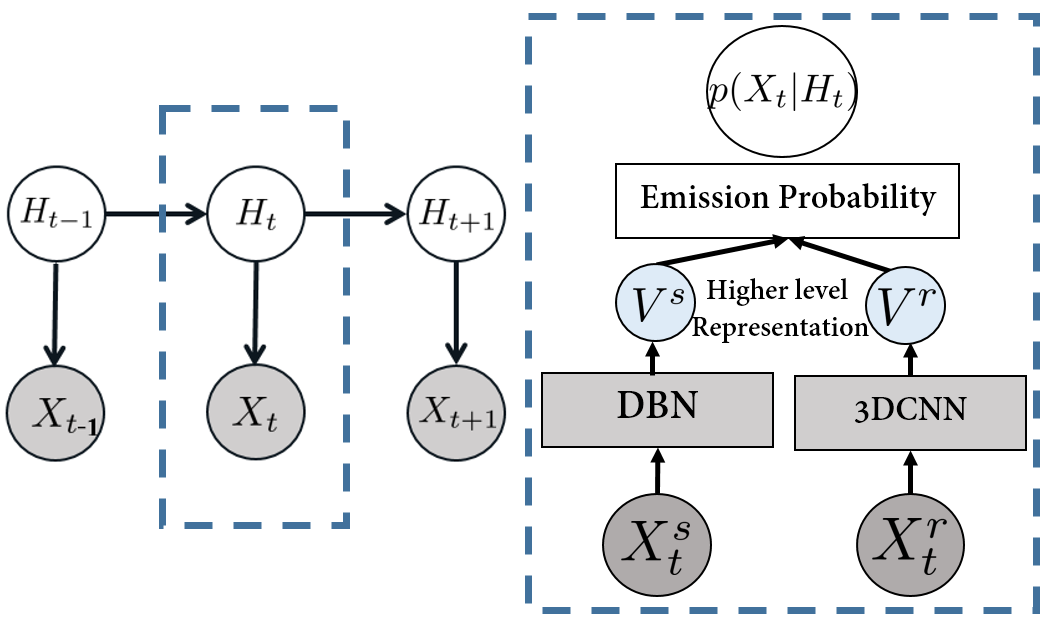
\includegraphics[width=0.45\textwidth]{images/GraphicalModel_new2}\\
  \caption{
 \small{ Gesture recognition model: the temporal model is a HMM (left), whose emission probability
\emissionprob{} (right) is modeled by forward-linked neural networks.
%%
More precisely, observations $\observation_t$ (skeletal features $\observationSK_t$, or RGB-D image features $\observationRGBD_t$)
are first passed through appropriate deep neural nets (a Deep Belief Network -\DBN- pretrained with Gaussian-Bernouilli Restricted Boltzmann Machines
for the skeleton modality, and
 a 3D convolutional neural network -\ThreeDCNN- for the \RGBD  modality) to implictly extract high-level features (\highSK and \highRGBD)
which are further fused to produce an estimate of $p(\observation_t|\hiddenstate_t)$.
}}
\label{fig:GM}
\end{figure}

Inspired by the framework successfully applied to speech recognition~\cite{mohamed2012acoustic}, the proposed model is a data driven learning system. This results in an integrated model, where the amount of prior knowledge and engineering is minimised. On top of that, this approach works without the need for additional complicated preprocessing and dimensionality reduction methods as it is naturally embedded in the framework.

The proposed approach relies on a Hidden Markov Model (HMM) for the temporal part,
and neural networks to model the emission probabilities.
 In the remainder of this section, we will first present our temporal model and then introduce its main component.
The details of the two distinct neural networks and fusion mechanisms along with post-processing will be provided
in Section~\ref{sec:ModelImplementation}.


\subsection{Deep Dynamic Neural Networks}
\label{sec:DDNN}

The proposed deep dynamic neural network \emph{(DDNN)} can be seen as an extension of~\cite{diwucvpr14}, where instead of only using the restricted Boltzmann machines to model human motion, various connectivity layers (fully connected layers, convolutional layers) are stacked together to learn higher level features justified by a variational bound~\cite{hinton2006fast} from different input modules.

A continuous-observation HMM  is adopted for modelling higher level temporal relationships.
At each time step $t$, we have one observed random variable $\observation_t$
composed of the skeleton input $\observationSK_t$ and RGB-D input images $\observationRGBD_t$
as shown in the graphical representation in Fig.~\ref{fig:GM}.
%
 The hidden state variable $\hiddenstate_t$ takes on values in a finite set  \finiteset composed of \numberhiddenstate states related to
the different gestures.
 The intuition motivating the HMM model is that a gesture is composed of a sequence of poses where the relative duration of each pose may vary.
This variance is captured by allowing flexible forward transitions within a Markov chain.
In practice,  $\hiddenstate_t$ can be interpreted as being in a particular phase  of a gesture \gesturea{}.

Classically under the HMM assumption, the joint probability of observations and states is given by:
\begin{equation}
p(H_{1:T},X_{1:T}) = p(H_1)p(X_1 | H_1) \prod^{T}_{t=2} p(X_t | H_t ) p(H_t | H_{t-1}),
\label{HMM_GM_1}
\end{equation}
where $p(\hiddenstate_1)$ is the prior on the first hidden state, $p(\hiddenstate_t|\hiddenstate_{t-1})$
is the transition dynamics modelling the allowed state transitions and their probabilities,
 and $p(\observation_t | \hiddenstate_t )$ is the emission probability of the observation,
modelled by  deep neural networks in our case. These elements are presented below.


%\subsection{Ergodic States Hidden Markov Model}

\begin{figure}[t]
  \centering
  % Requires \usepackage{graphicx}
  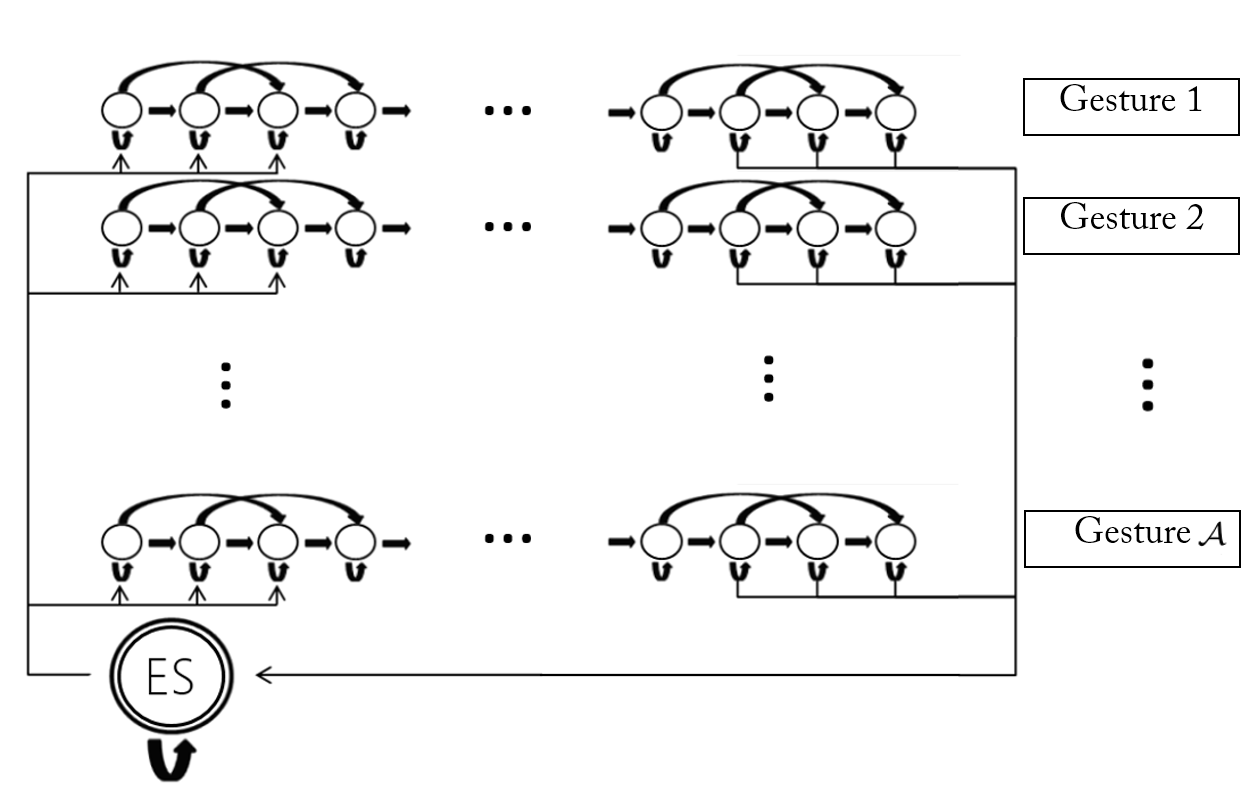
\includegraphics[width=0.45\textwidth]{images/HMM_2_new}\\
  \caption{
   \small{ State diagram of the \emph{ES-HMM} model for low-latency gesture segmentation and recognition. An ergodic state (\emph{$\mathcal{ES}$}) is used to model the resting position between gesture sequences. Each node represents a single state and each row represents a single gesture model. The arrows indicate possible transitions between states.}}
    \label{HMM_ES}
\end{figure}


\subsection{State-transition model and inference}
\label{sec:statemodel}


The HMM framework can be used for simultaneous gesture segmentation and recognition.
This is achieved by defining the state transition diagram as shown in Fig~\ref{HMM_ES}. For each given gesture $a \in \mathcal{A}$, a set of states $\mathcal{H}_a$ is introduced to defined a Markov model of that gesture. For example, for action sequence ``tennis serving", the action sequence can implictly be dissected into $\hiddenstatenode_{a_1}, \hiddenstatenode_{a_2}, \hiddenstatenode_{a_3}$ as: 1) raising one arm 2) raising the racket 3) hitting the ball.
More precisely, since our goal is to capture the variation in speed of the performed gestures, we set the transition matrix \transitionmatrix{}  in the following way: when being in a particular node $n$ at time $t$, moving to time $t + 1$, we can either stay in the same node (slower), move to node $n + 1$, or move to node $n+2$ (faster).
%
Furthermore, to allow the segmentation of gestures, we add an ergodic state
(\emph{$\mathcal{ES}$}) which resembles the silence state for speech recognition and which serve as a catch-all state.
From this state we can move to the first three nodes of any gesture class, and from the last three nodes of any gesture class we can move to $\mathcal{ES}$.
Hence, the hidden variable \hiddenvariable{} can take values within the finite set
 $\mathcal{H}=(\bigcup _{a \in \mathcal{A}} \mathcal{H}_a) \bigcup \{\mathcal{ES}\}$.

Overall, we refer to the model as the ergodic states hidden Markov model (\emph{ES-HMM}) for simultaneous gesture segmentation and recognition. It  differs from the firing hidden Markov model of~\cite{nowozin2012action} in that we strictly follow a left-right HMM structure without allowing backward transition, forbidding inter-states transverse, assuming that the considered gestures do not undergo cyclic repetitions as in walking for instance.


%The emission probability is represented as a matrix of size $N_{\mathcal{TC}} \times N_{\mathcal{F}}$ where $N_{\mathcal{F}}$ is the number of frames and output target class $N_{\mathcal{TC}}=N_{\mathcal{A}} \times N_{\mathcal{H}_a}+1$ where $N_{\mathcal{A}}$ is the number of gesture classes and $N_{\mathcal{H}_a}$ is the number of states associated to an individual gesture $a$ and one $\mathcal{ES}$ state (\emph{c.f.} Fig. \ref{Sample0700_comparison}: x-axis as $N_{\mathcal{F}}$ and y-axis as $N_{\mathcal{TC}} $ with $\mathcal{ES}$ as the bottom y-axis 101).


Once we have the trained model, we can use standard techniques to infer online the filtering
distribution $p(\hiddenstate_t | \observation_{1:t})$,  or offline (or with delay)
the smoothed distribution $p(H_t | X_{1:T})$ where $T$ denotes the end of the sequence.
Because the graph for the hidden Markov model is a directed tree, this problem can be solved exactly and efficiently using the max-sum algorithm also known as Viterbi algorithm. This algorithm searches the space of paths efficiently to find the most probable path with a computational cost that grows only linearly with the length of the chain~\cite{bishop2006pattern}.
%We can infer the gesture presence in a new sequence by Viterbi decoding.
% \begin{equation}
%    V_{t,\mathcal{H}}= \log P(X_t | H_t)+  \log(\max_{\mathcal{H} \in \mathcal{H}_a}( V_{t-1,\mathcal{H}}))
%    \label{viterbi_GDBN}
%\end{equation}
%whith the initial state $V_{1,\mathcal{H}}=P(X_1 |H_1)$.
%From the inference results, we define the probability of a gesture $a \in \mathcal{A}$ as $p(y_t=a|x_{1:t}) =V_{T,\mathcal{H}}$.
The result of the Viterbi algorithm is a path--sequence $\hat{\hiddenstatenode}_{t:T}$ of nodes going through the state diagram of
Fig.\ref{HMM_ES} and from which we can easily infer the class of the gesture as illustrated in Fig.~\ref{fig:Sample0700_comparison}.



\subsection{Learning the emission probability}
\label{sec:ProblemFormation}
\label{sec:emissionprob}

Traditionally, emission probabilities for activity recognition have been trained with Gaussian Mixture Models (GMM), one per state.
%
Alternatively, in this work we propose to model this term in a discriminative fashion.
More precisely, since the input features have a high dimensionality,
we propose to learn them using two distinctive types of neural networks each suited to the input modality,
as summarized in the right of Fig.~\ref{fig:GM}.
%

Unfortunately, estimating a probability density such as an emission probability remains quite a difficult problem, especially in high dimensions.
%
Theoretically, discriminative neural networks estimate posterior probabilities $p(\hiddenstate_t | \observation_t)$. We should divide posteriors by priors to get the scaled likelihoods which are required by the HMM for decoding. However, using scaled likelihood may not be beneficial if estimated priors do not match the priors in the test set \cite{morris2001multi}. Therefore, we employ the posteriors directly without dividing by the priors. This is equivalent to assuming that all priors are equal.
%
or, in other words, inference in the HMM only depends only on the ratio between emission probabilities for the different states. One can interpret that the models are trained to directly predict the ratio between emission probabilities. This is similar to the approach used by Kindermans et al. to integrate transfer learning and an HMM based language model into a single probabilistic model \cite{Kindermans2012a}.
One should think of the predicted emission probability ratio as an unnormalized version of the true emission probability. Nevertheless, to simplify the discussion of our models for readers with a basic understanding of HMMs, we will refer to the predicted emission probability ratio simply as emission probabilities since the underlying model remains unchanged.


For  the skeletal features, we rely on a Deep-Belief Network (DBN) trained in two steps \cite{salakhutdinov2009learning}:
in the first step,  stacked Restricted Boltzmann Machines (RBM) are trained in an unsupervised fashion using only observation data
to learn  high-level feature representations;
in the second step, the model is used as a Deep-Belief Network whose weights are further fine-tuned
for learning the emission probability.
%
For the RGB and depth (RGB-D) video data, we rely on a 3D (2D for space and 1D for time)
convolutional neural networks (3DCNN) to model the emission probabilities.
%
Finally, a fusion method combines in an intermediate or in a late stage the contributions of both modalities.
%
In all cases (including the fusion), the supervised training is conducted by learning to
predict the state label (an element of \finiteset) associated to each training or testing frame.


Such an approach present several advantages over the traditional GMM paradigm.
%
%Traditionally, GMMs and HMMs co-evolved as a way of doing speech recognition when computers were too slow to explore more computationally intensive approaches.
First, while  GMMs are easy to fit when they have diagonal covariance matrices and, with enough components,
can model any distribution, they have been shown to statistically inefficient at modeling high-dimensional features
with many componential structure as explained in~\cite{mohamed2012acoustic}.
%
For instance, assume that the components of the input feature space can be separated into two subspaces
characterized by  $N$  and $M$ significantly different  patterns in the training data, respectively, and that the occurences
of these patterns are relatively independent\footnote{In our case, intuitively these spaces could be the  features from different body parts,
like left/right arm or torso features.}.
%
A GMM will requires $N*M$ components to model this structure because each component must generate all the input features.
%
On the other hand, a stacked RBMs model that can explains the data using multiple causes only requires $N+M$ components
(in the ideal fully independent case), each of which is specific to a particular subspace.
%
This exponential inefficiency of GMMs at modeling factorial structures leads to GMM+HMM systems having
a very large number of Gaussians, most of which must be estimated from a very small fraction of the data.


Secondly, the approach for training the skeleton DBN model, first using variational learning to train stacked RBMs with unlabeled data, then in a discriminative fashion
\cite{salakhutdinov2009learning} has been shown to have several advantages.
%
It has been observed that  variational learning~\cite{hinton2006fast},
which tries to optimize the data-likelihood while minizing the Kullback-Leibler divergence between
the true posterior distribution of the hidden state (i.e. hidden layer variables of the RBMs  in our case)
and an approximation of this distribution, tends to produce unimodal distributions.
%
This is beneficial, as this means that similar sensory inputs will be mapped to  similar hidden variables.
%
Thus, the intuition for using DBN  for modeling the emission probability $p(\observation_t|\hiddenstate_t)$
from skeleton joints  is that by learning the multi-layer network layer by layer,
semantically meaningful high level features for skeleton configuration will be extracted while at the same
time a  parametric prior of human pose is learned.
%
%In the recent work of~\cite{6751269} a non-parametric bayesian network is adopted for human pose prior estimation, whereas in our framework, the parametric networks are incorporated.
%
In our case, using the pairwise joints features as raw input, the data-driven approach network will be able to extract relational
multi-joint features which are relevant to the target classes.
For instance, from  the ``toss" action data, a wrist joints rotating around shoulder joints feature is expected to
be extracted from the backpropagation  learning, and be the equivalent of those task specific \emph{ad hoc} hard wired sets
of joint configurations defined in~\cite{chaudhry2013bio}~\cite{muller2006motion}\cite{nowozin2012action}~\cite{ofli2013sequence}.

The benefit of such a learning approach is even more important when large amount of unlabelled data (e.g. skeleton data
 inferred from depth images of people performing unknown gestures) is available in addition to the labeled ones
(this was not the case in this paper).
%
%% The benefit of learning a generative model is greatly magnified when there is a large supply of unlabeled skeletal, RGB and depth data either acquired by motion capture systems or inferred from depth images in addition to the training data that has been labeled by a forced HMM alignment. We do not make use of unlabeled data in this paper, but it could only improve our results relative to purely discriminatively approaches.
%
Naturally, many of the  features learned in this unsupervised way might  be irrelevant for making the required discriminations,
even though they are important for explaining the input data.
However, this is a price worth paying if data availability and computation are cheap and
lead to  a stable mapping of the high-dimensional input  into high-level features
that are very good for discriminating between classes of interest.
%
In this view, it is important to notice that each weight in a neural network is usually constrained by a larger fraction of
the training samples than each parameter in a GMM, a point that has been masked by other differences in training.
In particular,  neural networks have traditionally been training discriminatively, whereas GMMs are typically trained as generative models,
%(even if discriminative training is performed later in the training procedure).
which given their parametric  nature  partially compensates the fact that each mixture
of a large GMM is usually trained on a very small fraction of the data.

In summary, the feed forward neural networks offer several potential advantages over GMMs:
\begin{itemize}
\item their estimation of emission  probabilities does not require detailed assumptions about the data distribution;
\item they allow an easy combination of diverse features, including both discrete and continuous features;
\item they use far more of the data to constrain each parameter because the output on each training case
is sensitive to a large fraction of the weights.
\end{itemize}



%% \textbf{Learning the higher level representation for skeleton joints features}: \label{skeleon_high_level}

%Neal and Hinton~\cite{neal1998view} demonstrated that the negative log probability of a single data vector, $\textbf{v}^0$, under the multi-layer generative model is bounded by a variational free energy, which is the expected energy under the approximating distribution, $Q(\textbf{h}^0 |\textbf{v}^0 )$, minus the entropy of that distribution. For a directed model, the ``energy" of the configuration $\textbf{v}^0 $,$\textbf{h}^0$ is given by $  E(\textbf{v}^0, \textbf{h}^0) = - [ \log p(\textbf{h}^0)+ \log p(\textbf{v}^0 | \textbf{h}^0)]$.
%% So the bound is
%% \begin{align*}
%%     \log p(\textbf{v}^0) &\geqslant \sum_{\textbf{h}^0} Q(\textbf{h}^0 | \textbf{v}^0) [ \log p (\textbf{h}^0) + \log p (\textbf{v}^0 | \textbf{h}^0)] \\
%%      &- \sum_{\textbf{h}^0} Q(\textbf{h}^0 | \textbf{v}^0) \log Q(\textbf{h}^0 |\textbf{v}^0)
%% \end{align*}

%% The intuition using deep belief networks for modeling marginal distribution \emissionprob{} in skeleton joints action recognition is that by constructing multi-layer networks, semantically meaningful high level features for skeleton configuration will be extracted whilst learning the parametric prior of human pose from mass pool of skeleton joints data. In the recent work of~\cite{6751269} a non-parametric bayesian network is adopted for human pose prior estimation, whereas in our framework, the parametric networks are incorporated.

%% Using the pair wise joints features as raw input, the data-driven approach network will be able to extract relational multi-joints features which are relevant to target frame class. E.g., for ``toss" action, wrist joints is rotating around shoulder joints would be extracted from the backpropagation via target frame as those task specific, \emph{ad hoc} hard wired sets of joints configurations as in~\cite{chaudhry2013bio}~\cite{muller2006motion}\cite{nowozin2012action}~\cite{ofli2013sequence}.

%% The outputs of the neural net are the hidden states learned by force alignment during the supervised training process.
%% Once we have model, we can use the normal online or offline smoothing, inferring the hidden marginal distributions of every node (frame) of the test video.

%The overall algorithm for training and testing are presented in Algorithm \ref{MMDDN_train} and \ref{MMDDN_test}.

%\begin{algorithm}
%\caption{Multimodal deep dynamic networks -- training}\label{MMDDN_train}
%\LinesNumbered
%\SetAlgoLined
%\SetAlgoNoEnd
%\DontPrintSemicolon
%\SetKwFunction{zeroes}{zeroes}
%\KwData{\;
%          \inputsequence=$[\framefeature_{i,1}, \ldots,\framefeature_{i,t},\ldots, \framefeature_{i,T}]$ \;
%          $ \mathbf{X^1=\{ x^1_i\}_{i \in [1 \ldots t]}}$ - raw input (skeletal) feature \; \hspace{1cm} sequence.\;
%          $ \mathbf{X^2=\{ x^2_i\}_{i \in [1 \ldots t]}}$ - raw input (depth) feature \; \hspace{1cm} sequence in the form of     $M_1 \times M_2 \times T$, where \; \hspace{1cm} $M_1, M_2$ are the height and width of the input \; \hspace{1cm} image and $T$  is the number of contiguous \; \hspace{1cm} frames of the spatio-temporal cuboid. \;
%          $ \mathbf{Y=\{ y_i\}_{i \in [1 \ldots t]}}$  - frame based local label (achieved by\; \hspace{1cm} semi-supervised forced-aligment), where \;
%          \hspace{1cm} $ \mathbf{y_i} \in \{ N_{\mathcal{A}} * N_{\mathcal{H}_a} + \textbf{\emph{1}} \} $ with $N_{\mathcal{A}}$ the number of \;
%          %\hspace{1cm} classes, $N_{\mathcal{H}_a$ is the number of hidden states for \; \hspace{1cm} each class,
%          \hspace{1cm} gesture classes and $N_{\mathcal{H}_a}$ is the number of \;
%          \hspace{1cm} states associated to an individual gesture $a$ \;
%          \hspace{1cm} and $\textbf{\emph{1}}$ as ergodic state.
%            }
%%\For{$m \leftarrow 1$ to $2$}{
%    \SetAlgoVlined
%    %\eIf{$m$ is $1$}{
%
%
%        Preprocess skeletal data $ \mathbf{X^1}$ as in Eq.\ref{sk_features_1}, \ref{sk_features_2}, \ref{sk_features_3}.\;
%        Normalise (zero mean, unit variance per dimension) the above features and feed it to Eq.\ref{GRBMenergy}. \;
%        Pre-train the networks using \emph{Contrastive Divergence}. \;
%        Supervised fine-tuning of the deep belief networks using $ \mathbf{Y}$ by standard mini-batch \emph{SGD} backpropagation.\;
%    %}{
%        Preprocess the depth and RGB data $ \mathbf{X^2}$ as in \ref{3d_preproc}.\;
%        Feed the above features to Eq.\ref{ReLU}. \;
%        Train the 3D convolutional neural networks using $ \mathbf{Y}$.\;
%    %}
%%}
%\KwResult{\;
%        $\mathbf{GDBN}$ - a Gaussian-Bernoulli visible layer deep \;
%                \hspace{1cm} belief network to generate the emission \;
%                \hspace{1cm} probabilities for the hidden Markov model.\;
%        $\mathbf{3DCNN}$ - a 3D deep convolutional neural \;
%                    \hspace{1cm} network to generate the emission probabilities\;
%                    \hspace{1cm} for the hidden Markov model.\;
%        $\mathbf{p(X_t | H_t )}$ emission probability. \;
%        $\mathbf{p(H_1)}$ - prior probability for $ \mathbf{Y}$ by accumulating and \;
%                \hspace{1cm} normalising labels.\;
%        $ \mathbf{p(H_t | H_{t-1})}$ - transition probability for $ \mathbf{Y}$,  enforcing\;
%                \hspace{1cm} the beginning and ending of a sequence can \;
%                \hspace{1cm} only start from the first or the last state.
%}
%\end{algorithm}
%%%%%%%%%%%%%%%%%%%%%%%%%%%%%%%%%%%%%%%%%%%%%%%%%%%%%%%%%%%%%%%%%%%%%%%%%%%%%%%%%%%%%%%%%%%%%%%%%%%%%%%%%%%%%%%%%
%\begin{algorithm}[t]
%\caption{Multimodal deep dynamic networks -- testing}\label{MMDDN_test}
%\LinesNumbered
%\SetAlgoLined
%\SetAlgoNoEnd
%\DontPrintSemicolon
%\SetKwFunction{zeroes}{zeroes}
%\KwData{\;
%         $\mathbf{X^1=\{x^1_i\}_{i \in [1 \ldots t]}}$ - raw input (skeletal) feature \; \hspace{1cm} sequence.\;
%         $\mathbf{X^2=\{x^2_i\}_{i \in [1 \ldots t]}}$ - raw input (depth) feature \; \hspace{1cm} sequencein the form of $M_1 \times M_2 \times T$. \;
%         $\mathbf{GDBN}$ - trained Gaussian-Bernoulli visible layer  \;
%                \hspace{1cm} deep belief network to  generate the emission\;
%                 \hspace{1cm} probabilities for the hidden Markov model.\;
%         $\mathbf{3DCNN}$ - trained  3D deep convolutional neural\;
%                    \hspace{1cm} network to generate the emission\;
%                    \hspace{1cm} probabilities for the hidden Markov model.\;
%        $\mathbf{p(H_1)}$ - prior probability for $ \mathbf{Y}$.\;
%        $ \mathbf{p(H_t | H_{t-1})}$ - transition probability for $ \mathbf{Y}.$
%            }
%
%%\For{$m \leftarrow 1$ to $2$}{
%    \SetAlgoVlined
%    %\eIf{$m$ is $1$}{
%        Preprocessing and normalising the skeletal data $ \mathbf{X^1}$  as in Eq. \ref{sk_features_1}, \ref{sk_features_2}, \ref{sk_features_3}.\;
%        Feedforwarding network $\mathbf{GDBN}$ to generate the emission probability $\mathbf{p(X_t | H_t )}$ in Eq.\ref{HMM_GM_1}. \;
%        Generating the score probability matrix $\mathbf{S^1 = p(H_{1:T},X_{1:T}).}$ \;
%    %}{
%        Preprocessing(median filtering the depth data) and normalising data RGB-D data $ \mathbf{X^2}$ .\;
%        Feedforwarding $\mathbf{3DCNN}$ to generate the emission probability $\mathbf{S^2 = p(X_t | H_t )}$ in Eq.\ref{HMM_GM_1}. \;
%        Generating the score probability matrix $\mathbf{S^2 =p(H_{1:T},X_{1:T}).}$ \;
%    %}
%%}
%        Fuse the score matrix $\mathbf{S = \alpha * S^1 + (1-\alpha)* S^2}$ OR the learnt joint representation.\;
%        Finding the best path $\mathbf{V_{t,\mathcal{H}}}$ using $\mathbf{S}$ by Viterbi decoding. \;
%\KwResult{\;
%        $ \mathbf{Y=\{ y_i\}_{i \in [1 \ldots t]}}$  - frame based local label  \;
%        $ \mathbf{C}$ - global label, the anchor point is chosen as the\;
%                        \hspace{1cm} middle state frame.\;
%}
%\end{algorithm}



\endinput


%%%%%%%%%%%%%%%%%%%%%%%%%%%%%%%%%%%%%%%%%%%%%%%%%%%%%%%%%%


\section{Model Implementation}
\label{sec:ModelImplementation}

In this section, we detail the different component of the proposed Deep Dynamic Neural Network approach.

\subsection{Ergodic States Hidden Markov Model}

In all our experiments, the different modelling elements are specified as follows.

The number of states \nsig{} associated to an individual gesture has been set to 5.
In total, the number of states is $\tns = 20 \times 5 + 1 = 101$
when conducting  experiments on the Chalearn dataset containing 20 classes.
%
Note that intuitively, 5 states represents a good granularity as
most gestures in the dataset are composed of 5 phases: an onset, followed by arm motions to reach a more or less static pose (often characterized by a distinct hand posture), and the motion back to the resting position.
%
In future work, the optimisation of the number of states\footnote{Experiments with 10 states led to similar performance.} and even a different number of states per gesture could be investigated.
%


The training data of the Chalearn competition is given as a set of sequences
$\inputsequence_i=[\framefeature_{i,1}, \ldots,\framefeature_{i,t},\ldots, \framefeature_{i,T_i}]$
where $\framefeature_{i,t}=[\framefeature_{i,t}^s, \framefeature_{i,t}^r]$. Here,  $\framefeature_{i,t}^s$ corresponds to the skeleton and $\framefeature_{i,t}^r]$ denotes the RGB-D input.
%
As only a single gesture label is provided for each sequence, we need to define
$\labelsequence_i=[\framelabel_{i,1}, \ldots,\framelabel_{i,t},\ldots, \framelabel_{i,T_i}]$,
the sequence of state labels $\framelabel_{i,t}$ associated to each frame.
%
To do so, a forced alignment is used. This means that if the $i^{th}$ sequence is a gesture \gesturea{}, then the first $\lfloor \frac{T_i}{5} \rfloor$ frames are assigned to state $\hiddenstatenode_\gesturea^1$ (the first state of gesture \gesturea{}),
the following $\lfloor \frac{T_i}{5} \rfloor$ frames are assigned to $\hiddenstatenode_\gesturea^2$, and so forth.

Note that each gesture sequence comes with the video frames preceding and following the gesture.
In practice, we extracted 5 frames before and after each gesture sequence and labelled them
%this shot sequence
with the ergodic state (\ergodicstate) label.
%
The transitional matrix \transitionmatrix{} was learned by simply  collecting the transition statistics from the label sequences $\labelsequence_i$, allowing 5 frame jumps to accommodate skipping states.

% \begin{flushleft}
%\textbf{\emph{Hidden states} ($\mathcal{H}_a$): } Force alignment is used to extract the hidden states, \emph{i.e.} if a gesture token is 100 frames, the first $20= \frac{100}{5(N_{\mathcal{H}_a} )}$ frames are assigned to hidden state $\textbf{\emph{1}}$, the following 20 frames are assigned to hidden state $\textbf{\emph{2}}$, and so forth.
%
%\textbf{\emph{Ergodic states ($\mathcal{ES}$)}:} Neutral frames are extracted as 5 frames before or after a gesture token, according to the ground truth labels.
%
%\textbf{\emph{Transitional Matrix (\transitionmatrix{})}:} Statistics is collected from the labelling stage, allowing 5 frame jumps to accommodate skipping states.
%\end{flushleft}


\subsection{Skeleton Module}
\label{sec:skeleton_module}


%\begin{figure}[t]
%  \centering
%  % Requires \usepackage{graphicx}
%  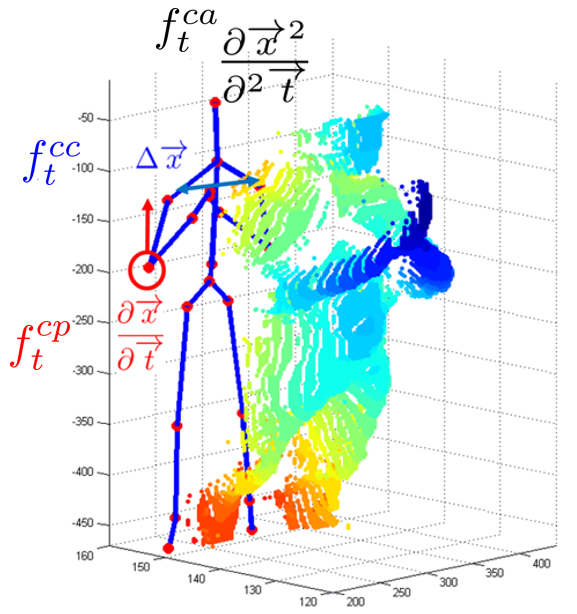
\includegraphics[width=0.3\textwidth]{images/point_cloud}\\
%  \caption{
%    A point cloud projection of a depth image and the 3D positional features.}
%    \label{point_cloud}
%\end{figure}
%
%
%\begin{figure}[t]
%  \centering
%  % Requires \usepackage{graphicx}
%  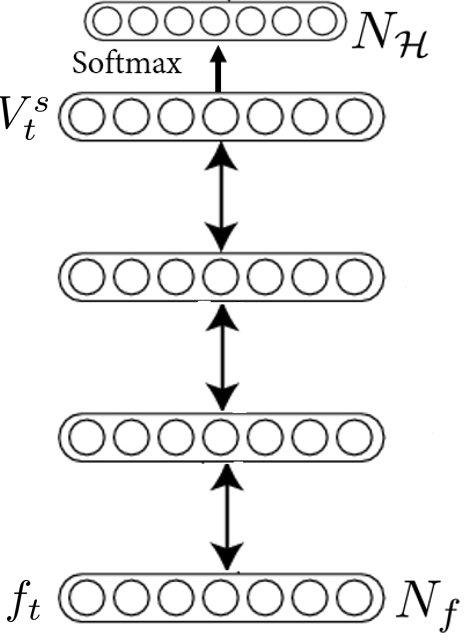
\includegraphics[width=0.23\textwidth]{images/DBN}\\
%  \caption{
%  A \DBN is trained to predict the emission probability  $p(\observationSK_t|\hiddenstate_t)$
%  from the  skeleton input \skfeature.
%  The double arrows indicate that the intermediate weights are first trained in an unsupervised fashion using stacked RBMs.
%}
%    \label{fig:DBN}
%\end{figure}


%\setlength{\fboxsep}{1pt}%
%\setlength{\fboxrule}{1pt}%
\begin{figure}[t]
       \centering
        \begin{subfigure}[c]{0.2\textwidth}
        \centering
                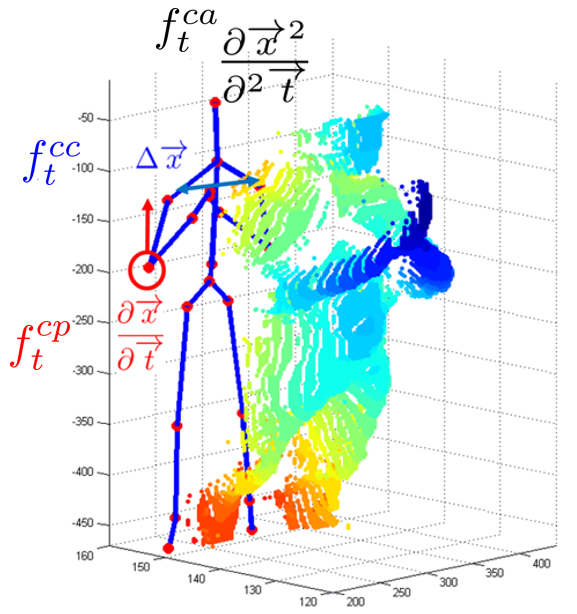
\includegraphics[width=4.5cm,height=5cm, clip]{images/point_cloud}
        \end{subfigure}%
        \hfill
        \begin{subfigure}[c]{0.2\textwidth}
        \centering
                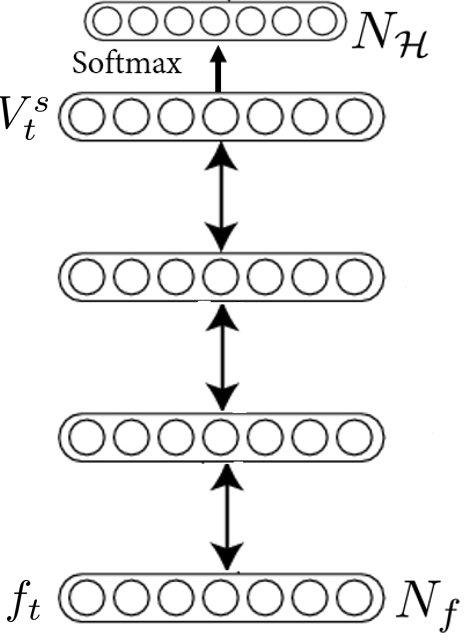
\includegraphics[width=4cm,height=5cm, clip]{images/DBN}
                %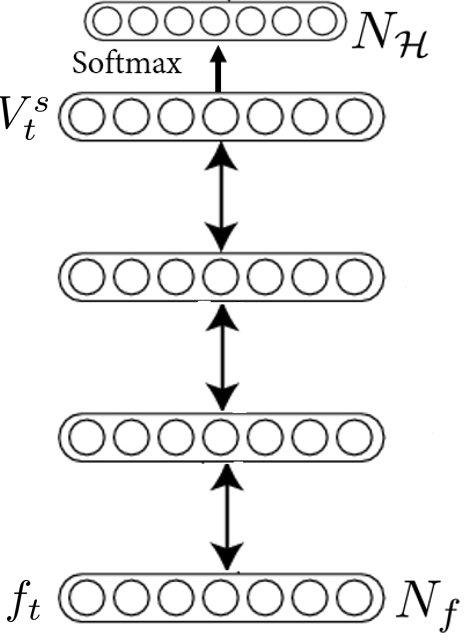
\includegraphics[width=0.2\textwidth]{images/DBN}
                %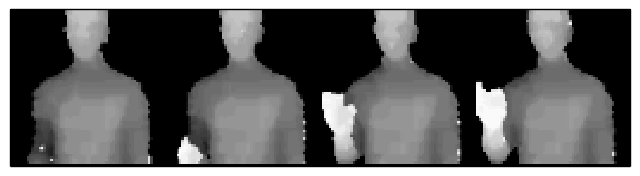
\includegraphics[width=2cm,height=3cm, trim=120 100 100 50, clip]{images/3dcnn_filters/original_images_depth_body_ok}
        \end{subfigure}
  \caption{
\small{ Left: A point cloud projection of a depth image and the 3D positional features.
  Right: A \DBN is trained to predict the emission probability  $p(\observationSK_t|\hiddenstate_t)$
  from the  skeleton input $\skfeature_t$.
  The double arrows indicate that the intermediate weights are first trained in an unsupervised fashion using stacked RBMs.
  }}
  \label{fig:DBN}\label{point_cloud}
\end{figure}


\subsubsection{Skeleton input features}

Given our task, only  the $\numberofjoints=11$ upper body joints are relevant and
considered, namely \emph{``ElbowLeft, WristLeft, ShoulderLeft, HandLeft, ElbowRight, WristRight, ShoulderRight, HandRight, Head, Spine, HipCenter"}.
%
The raw skeleton features of time $t$ are defined as $\skrawfeature_t=[\framefeature_t^{s,1}, \ldots, \framefeature_t^{s, \numberofjoints}]$.
To capture the gesture dynamics, rather than using $\skrawfeature_t$ as raw input to our data driven approach,
we follow the approach of~\cite{diwucvpr14} and compute the 3D positional pairwise differences of joints, as well as temporal derivatives, defined as (shown in Fig.~\ref{point_cloud}) \footnote{Note that the offset features used in~\cite{diwucvpr14} depend on the first frame.
Thus if the initialisation fails which is a very common scenario, the feature descriptor will be generally very noisy.
Hence, we do not use these offset features here.}:
\begin{align}
f^{cc}_t&=\{x_t^{s,i}-x_t^{s,j} | i,j=1,2,\ldots, N_j; i\neq j\} \label{sk_features_1}\\
f^{cp}_t&=\{x_{t+1}^{s,i}-x_t^{s,i} |  i=1,2,\ldots, N_j\} \label{sk_features_2}\\
f^{ca}_t&=\{x_{t+1}^{s,i} - 2 \times x_t^{s,i} + x_{t-1}^{s,i} | i=1,2,\ldots, N_j  \} \label{sk_features_3}
\end{align}
%
This results in an input feature vector $\skfeature_t=[f^{cc}_t, f^{cp}_t, f^{ca}_t]$ of dimension $N_{\skfeature}=N_j \times( \frac{ N_j}{2} + N_j + N_j)*\mathit{3}=891$.
Admittedly, here we do not completely neglect human prior knowledge about information extraction for relevant static postures, velocity and acceleration of overall dynamics of motion data.
While we have indeed used prior knowledge to define our relevant features, we believe they remain quite general and do not need dataset specific tuning.
Note that the feature extraction process resembles the computation of the
\emph{Mel Frequency Cepstral Coefficients (MFCCs)} and their temporal derivatives
typically used in the  speech recognition community~\cite{mohamed2012acoustic}.
%\textbf{\emph{Caveat}}:
%\begin{itemize}
%\item  When extracting skeletal features, the 3D joint coordinates have not been transformed from the world coordinate system to a person centric coordinate system by placing the \emph{``HipCenter"} at the origin.
%\item  Note also that the normalization scheme by scaling the skeleton position using length of \emph{``HipCenter"} and \emph{``Spine"} didn't work well in the implementation.
%\item The third point worth noting is that some actors performed gestures using left hand as a dominant hand whereas some using right hand which worth investigating the effect of this in the future. However, those tokens are treated indiscriminately.  Hence, the feature fed into \emph{GRBM} are almost raw, un-preprocessed.
%\end{itemize}

\subsubsection{Modeling \randomvariableSK{} using Deep Belief Networks}


%We briefly introduce the building elements of the network and a more detailed introduction can be found at:
%Boltzmann Machines (BMs) are a special structure of Markov Random Field (MRF), \emph{i.e.} the energy function is linear in term of its corresponding free parameters.
%To empower the expressiveness of the model so as to encode complex distributions, the hidden variables are introduced to enhance the modelling capability of the Boltzmann Machinesd with a two-layer structure, has the visible binary stochastic units $v\in \{0,1\}^D$ connected to the hidden binary stochastic units $h\in \{0,1\}^F$.
%
%The energy of the state $\{v,h\}$is:
%\begin{eqnarray}
%E(v,h;\theta)&=&-v ^{\top}Wh-b^{\top}v-a^{\top}h  \\
%             &=&-\sum^D_{i=1} \sum^F_{j=1} W_{ij} v_i h_j -\sum^D_{i=1}b_iv_i - \sum^F_{j=1}a_jh_j
%   \label{energy}
%\end{eqnarray}
%where $\theta=\{W,b,a\}$ are the free parameters: $W_{i,j}$ serves as the symmetric synergy term between visible unit $i$ and hidden unit $j$; $b_i$ is the bias term of the visible units and $a_j$ is the bias term of the hidden units.
%The joint distribution over the visible and hidden units is defined by:
%\begin{eqnarray}
%    P(v,h;\theta)&=&\frac{1}{Z(\theta)} \exp(-E(v,h;\theta)); \\
%        Z(\theta)&=&\sum_v \sum_h exp(-E(v,h;\theta))
%    \label{RBM}
%\end{eqnarray}
%The conditional distributions needed for inference and generation are given by:
%\begin{eqnarray}
%    P(h_{j=1}|\textbf{v})&=&g(\sum_i W_{ij}v_i+a_j)); \\
%      P(v_{i=1}|\textbf{h})&=&g(\sum_j W_{ij}h_j+b_i))
%\end{eqnarray}
%where $g(x)=\frac{1}{1+exp(-x)}$ is the logistic function.

%The derivative of the log-likelihood with respect to the model parameter from Eq.~\ref{RBM} is expressed as: $E_{P_{data}}[vh^{\top}]-E_{P_{model}}[vh^{\top}]$ where $E$ denotes the expectation.
%Due to the intractability of the second term, an approximation is generally required. This approximation is called the ``Constrative Divergence":
%%In practice, learning is done by following an approximation to the gradient of a different objective function, called the ``Constrative Divergence":
%\begin{equation}
%    \Delta W = \alpha (E_{P_{data}}  [\textbf{vh}^T]-E_{P_T}[\textbf{vh}^T]). \label{CD1}
%\end{equation}
%where $\alpha$ is the learning rate and $P_T$ is the distribution obtained by running a Gibbs chain, initialized with the visible units given by the data, for $T$ full steps.

Given the input skeleton feature \skfeature, a \DBN model is used to predict the emission probability, as shown in Fig.~\ref{fig:DBN}.
 The learning proceeds in two steps which we briefly mentioned in Section~\ref{sec:emissionprob}:
in the first step, the network is considered to be a stack of RBMs, and trained using a greedy, layer-by-layer
unsupervised learning algorithm \cite{hinton2006fast};
in the second step, a softmax network layer is added on top of the RBMs to create a \DBN architecture,
where the  weights of the first step are used to initialize the corresponding weights in the \DBN.
The \DBN is subsequently fine-tuned in a supervised manner to predict the emission probability.
%
The number of nodes at each layer of the \DBN are $[N_{\skfeature},2000,2000,1000,\numberhiddenstate]$.
% where $N_f = 891$ is the observation domain dimensionality; $N_{\mathcal{H}}$ is the output target class.
Below we give further details on the model and the training process.

\mypartitle{Gaussian-Bernoulli RBM.}
%
Restriced Boltzmann machine (RBM) are undirected graphical models involving visible and hidden variables,
with symmetric connections between the hidden and visible units of adjacent layers but without connections between units within the same layer.
%
In most cases, the units in the RBMs model binary random variables.
%
However, in our case the visible unit in the first layer contains the vector of skeleton features $\skfeature \in \mbf{R}^{N_{\skfeature}}$, whose values are continuous.
To be able to process this data, we resort to a Gaussian-Bernoulli RBM (\emph{GRBM})~\cite{salakhutdinov2009learning}.
The main difference w.r.t. a standard RBM lies in the following:
the energy term of the first layer $\skfeature$ to the hidden binary stochastic units $\rbmh \in \{0,1\}^F$ is given by:
\begin{equation}
    E(\skfeature,\rbmh;\theta) =-\sum_{i} \frac{(\skfeatureel_i-b_i)^2}{2\sigma_i^2} -\sum_{i} \sum_{j} W_{ij}  \rbmhel_j \frac{\skfeatureel_i}{\sigma_i}- \sum_{j=1}a_j\rbmhel_j
\label{GRBMenergy}
\end{equation}
where $\theta=\{W,b,a\}$ are the free parameters. Here $W_{i,j}$ serves as the symmetric synergy term between visible unit $i$ and hidden unit $j$.
The variables $b_i$ and $a_j$ specify the bias term of the visible and hidden units, respectively.
%
The conditional distributions needed for inference and generative modelling are given by the traditional logistic function $g$ for the binary hidden units, and the normal distribution $\mathscr{N}$  for the continuous units:
\begin{eqnarray}
    P(\rbmhel_j=1 | \skfeature) & = & g (\sum_i W_{ij} \skfeatureel_i+a_j) \\
    P(\skfeatureel_i=\skfeatureel|\rbmh) & = & \mathscr{N}( \skfeatureel |\mu_i,\sigma_i^2).
\end{eqnarray}
where $\mu_i=b_i+\sigma_i^2 \sum_j W_{ij}$.
In practice, we normalise the data (mean subtraction and standard deviation division) in the preprocessing phase.
Hence, instead of learning $\sigma_i^2$, one typically uses  $\sigma_i^2=1$ during training.

We ran 100 epochs using a fixed recipe based on stochastic gradient descent with a mini-batch size of 200 training cases
to train  the stacked RBM. The learning rate is fixed to 0.001 for the Gaussian-Bernoulli RBMs,
and to 0.01 for the higher-layer binary-binary RBMs.






\mypartitle{\DBN forward training.}
%
% In the training set, there are in total $400\,117$ frames. During the training of the \emph{DBN}, $90\%$ is used for training, $8\%$ for validation (for the purpose of early stopping) $2\%$ is used for test evaluation.
%
The \DBN is initialized with the result of the previous pre-training. The goal of this initialisation is to avoid suboptimal local minima and to increase
the network's generalisation capabilities.
The learning rate for the parameter fine tuning
starts at 1 with 0.99999 mini-batch scaling. During the experiments, early stopping occurs around epoch 440.
The optimisation completes with a frame based validation error rate of $16.5\%$.%, as shown in  Fig~\ref{sk_error_rate}.

% Although that further optimising the network architecture would lead to more competitive results, in order not to overfit, ``as algorithms over time become too adapted to the data set, essentially memorising all its idiosyncrasies, and losing ability to generalise"~\cite{torralba2011unbiased}, we would like to treat the model as the aforementioned more generic approach.
% Since a completely new approach will initially have a hard time competing against established, carefully fine-tuned methods.
%More fundamentally, it may be that the right way to treat dataset performance numbers is not as a competition for the top place.
%This way, fundamentally new approaches will not be forced to compete for top performance right away, but will have a chance to develop and mature.
%The performance of the skeleton module is shown in Tab.~\ref{Table_score_fusion}.

%\begin{figure}[t]
%  \centering
%  % Requires \usepackage{graphicx}
%  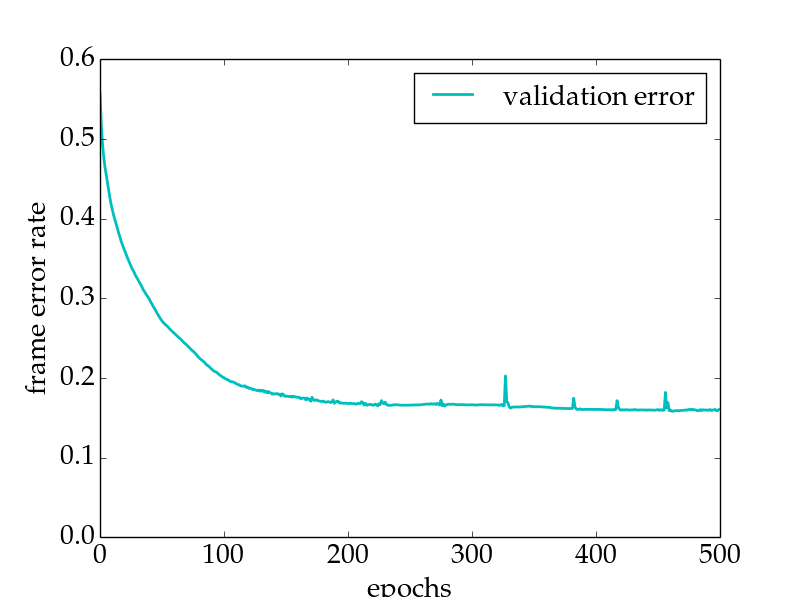
\includegraphics[width=0.4\textwidth]{images/sk_training_error}\\
%  \caption{
%    \small{Deep Belief Network frame based validation error rate for the skeleton modality.}
%%    The 0.05 frame error rate indicates the good generalisation property of the DBN skeleton module.
%    }
%    \label{sk_error_rate}
%\end{figure}

\subsection{RGB \& Depth 3D Module} \label{sec:rgbd_modules}
\subsubsection{Preprocessing}\label{3d_preproc}
\begin{figure*}[t]
  \centering
  % Requires \usepackage{graphicx}
  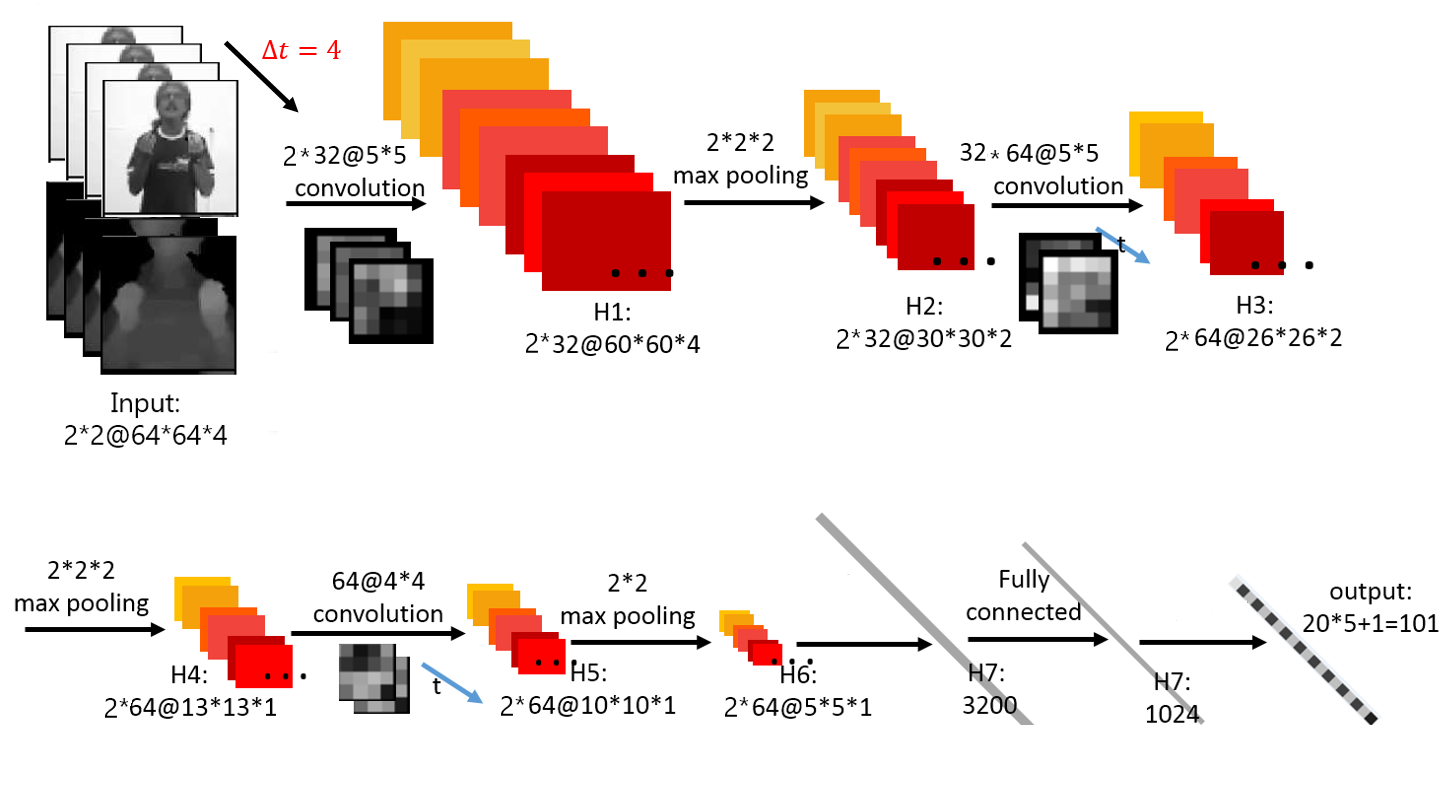
\includegraphics[width=.9\textwidth]{images/3DCNN_new}
\vspace*{-2mm}
  \caption{3DCNN architecture. The input is $2\times2@64\ast64\ast4$, meaning 2 modalities (depth and RGB)  for the hand and body regions,
each  being 4  consecutive 64 by 64 frames stacked together. See text for further details.
%
%Note that in H1, the Depth and RGB  response maps of the hand (and body) are summed to produce a single feature map,
%while in H7, the hand and body part feature maps of H6 are just flattened.
}
\label{3dcnn_architecture}
\end{figure*}
DeepMind ~\cite{mnih2013playing} presented the first deep learning model to successfully learn control policies directly from high-dimensional sensory input using deep reinforcement learning. However,  working directly with raw input Kinect recorded data frames, which are $640 \times 480$ pixel images, is computationally very demanding.
Therefore, our first step in the preprocessing stage consists of cropping the image to the highest hand and the upper body based on the given joint information. In the Chalearn dataset, we determined that the highest hand is the most interesting. When both hands are used, they tend to perform the same (mirrored) movement, When only one hand is used, it is always the highest one which is relevant for the gesture.
Furthermore, to be invariant to handedness, we train the model with the right hand view.
For this reason,  the video was mirrored when the left hand is actually the performing hand.


The preprocessing results in four video samples (body and hand with grayscale and depth) of resolution $64\times64$.
Furthermore, the noise in the depth maps is reduced by removing the background using the automatically produced
segmentation mask provided with the data, and applying a  median filtering.
%
Depth images are Z-normalised (the mean is subtracted -as it is rather irrelevant to the gesture subclass-
and the result divided by the standard deviation), whereas
RGB images are only normalized by the image standard deviation.
The outcome is illustrated in Fig.~\ref{3dcnn_filters}.
%\begin{figure}[t]
%  \centering
%  % Requires \usepackage{graphicx}
%  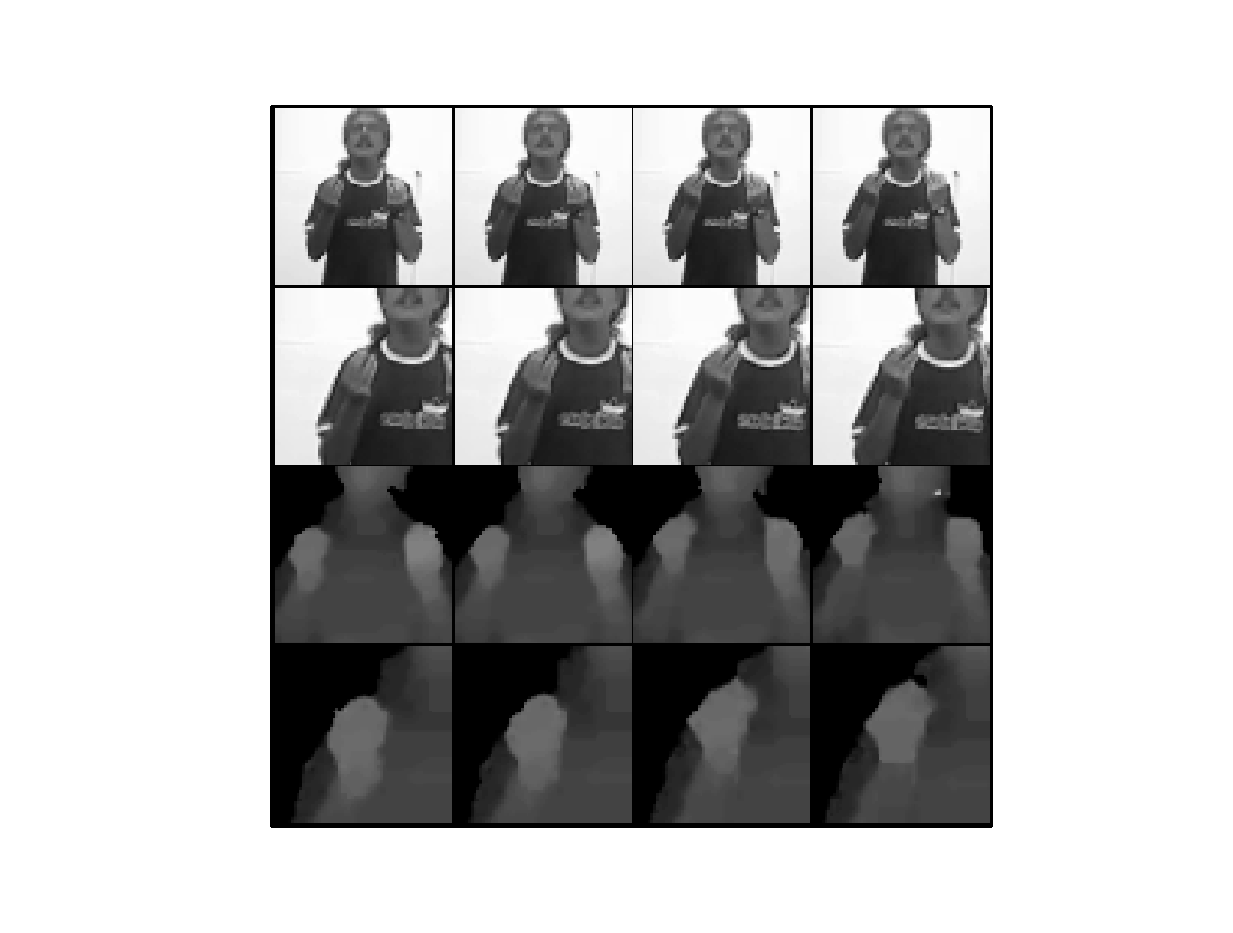
\includegraphics[width=0.5\textwidth]{images/3dcnn_filters/original.eps}\\
%  \caption{
%    Preprocessing result. Inputs  from top to bottom: 1) grayscale body input, 2) grayscale hand input, 3) depth body input, 4) depth hand input. }
%    \label{3dcnn input}
%\end{figure}


\subsubsection{3DCNN Architecture}
\label{sec:3dcnnArchitecture}

This  architecture consists of a series of layers composed of either convolution, pooling or, in the last layer, fully connected layers.
The 3D convolution itself is achieved by convolving a 3D kernel to the cuboid formed by stacking multiple contiguous frames together.
We follow the nomenclature of ~\cite{ji20133d}.
However, instead of using $tanh$ units~\cite{ji20133d},  Rectified Linear Units (\emph{ReLUs})~\cite{krizhevsky2012imagenet}
were used to speed up training.
Formally, the value of a unit at position $(x, y, z)$ ($z$ here corresponds to the time-axis) in the $j$-th feature map in the $i$-th layer, denoted as $v^{xyz}_{ij}$, is given by:
\begin{equation}
v^{xyz}_{ij} =  max( 0,  ( b_{ij} + \sum_m \sum_{p=0}^{P_i - 1} \sum_{q=0}^{Q_i -1 } \sum_{r=0}^{R_i -1} w^{pqr}_{ijm} v^{(x+p)(y+q)(t+r)}_{(i-1)m} ))
\label{ReLU}
\end{equation}
%
The complete 3DCNN architecture is depicted in Fig.~\ref{3dcnn_architecture}:
4 types of input contextual frames are stacked as size $64\times64\times4$ (as illustrated in Fig.~\ref{3dcnn_filters}).
%
The first layer (H1) consists of 32 feature maps produced by $5\times5$ spatial convolutional kernels,
followed by local contrast normalisation (LCN)~\cite{jarrett2009best}.
%
Note that the filter response maps of the Depth and RGB images of the hand (and body) are summed to produce a single feature map,
thus resulting in H1 32 feature maps for each of the hand and for the body region.
%
A 3D max pooling with strides $(2,2,2)$ is then applied.
%
The second layer uses 64 feature maps with $5\times5$ kernels followed by LCN and 3D max pooling with strides $(2,2,2)$.
The third layer is composed of 64 feature maps with $4\times4$ kernels followed by 3D max pooling with strides $(1,2,2)$.
All hand and body convolutional layer outputs of H6 are flattened in H7, and fed into one fully connected layer of size $1024$.
%
Finally, the output layer has \numberhiddenstate values, the number of states in the HMM state diagram (see Fig.~\ref{HMM_ES}).




\subsubsection{Details of Learning}
% The first 650 batches are used for training and the remaining 50 files for validation.
During training, dropout \cite{hinton2012improving} is used as the main regularisation approach to reduce overfitting.
Nesterov’s accelerated gradient descent (NAG) \cite{sutskever2013importance} with a fixed momentum-coefficient of 0.9 and mini-batches of size 64 are also used.
The learning rate is initialised at 0.003 with a 5\% decrease after each epoch. The weights of the 3DCNNs are randomly initialised from a normal distribution with $\mu = 0$ and $\sigma = 0.04$.
The frame based validation error rate is $39.06\%$ after 40 epochs. % as shown in Fig.~\ref{fig:RGBErrorRate}.
Compared with the skeleton module (16.5\% validation error rate), the 3DCNN has a notable higher frame based error rate.


%\begin{figure}[t]
%  \centering
%  % Requires \usepackage{graphicx}
%  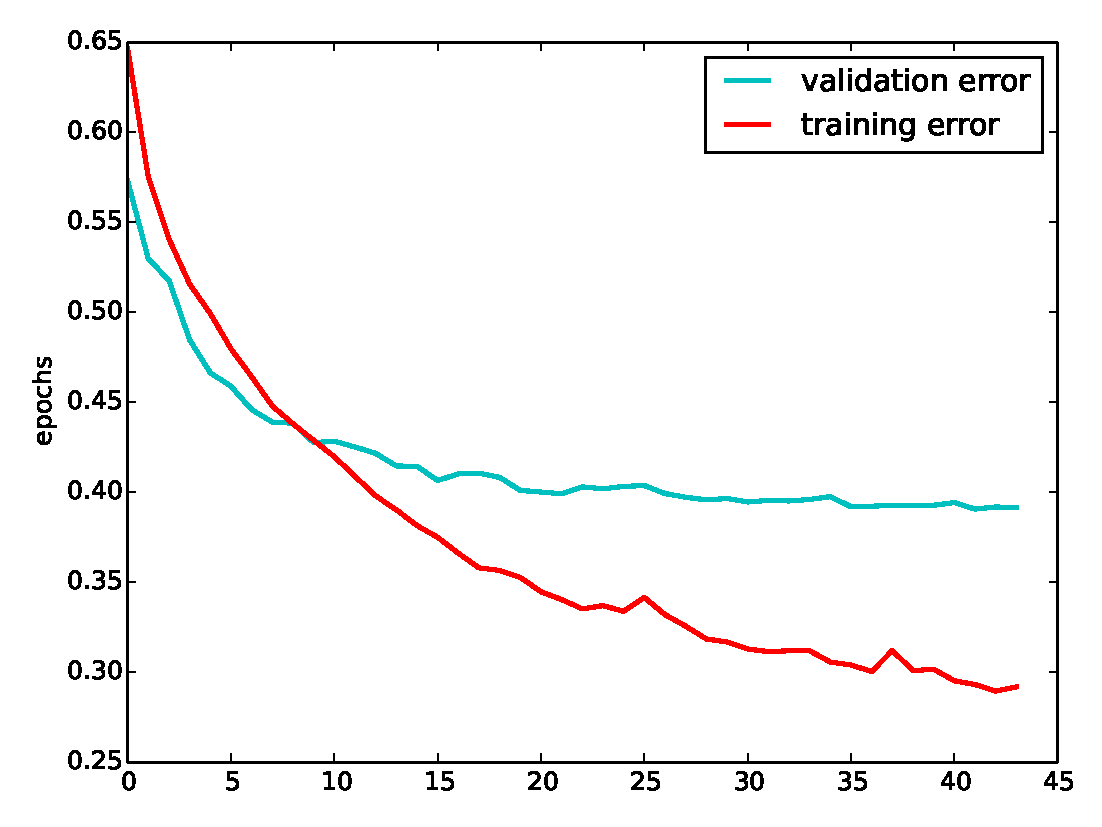
\includegraphics[width=.4\textwidth]{images/3dcnn_filters/training_error}
%  \caption{
%  \small{Frame based error rate of the 3DCNN.
% The error rates are much higher than when using the skeleton module (see Fig.~\ref{sk_error_rate})
% indicating that  learning from images is more difficult. }}
%\label{fig:RGBErrorRate}
%\end{figure}

\subsubsection{Looking into the Networks: Visualisation of the Filter Banks}

The convolutional filter weights of the first layer are depicted in Fig.~\ref{3dcnn_filters}.
The unique characteristics from the kernels are clearly visible: as hand input images (RGB and depth) have larger homogenous areas
than the body inputs, the resulting filters are smoother than their body-processing counterparts.
In addition to being smoother overall than the grayscale filters, depth filters also exhibit stronger edges. A similar finding was reported in~\cite{socher2012convolutional}.
%
Finally, when looking at the joint depth-image response maps, we  notice that some filters better capture segmentation-like information, while others are more edge-oriented.

\begin{figure*}[t]
  \centering
  % Requires \usepackage{graphicx}
  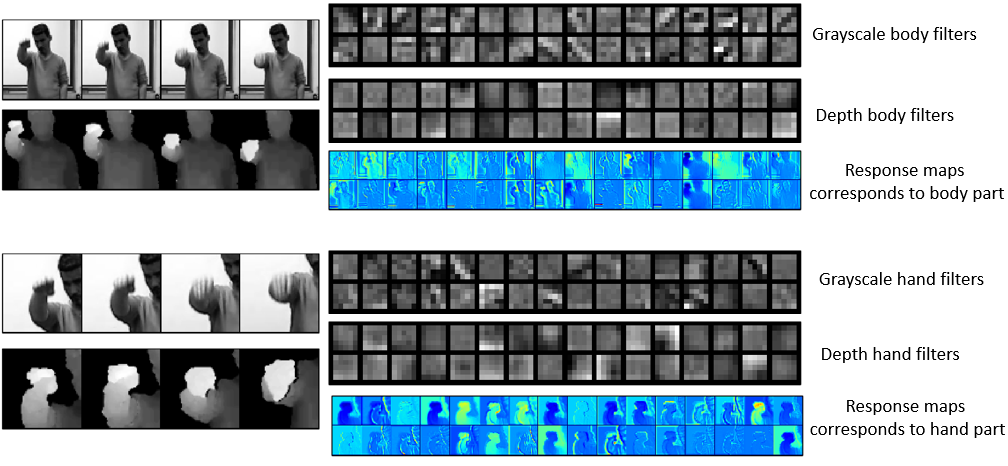
\includegraphics[width=0.85\textwidth]{images/CNN_filters}
  \caption{
  \small{Visualisation of input frames, first convolutional layer $5\times5$ filters, and corresponding response maps.
As depth images are smoother than the grayscale ones, the corresponding filter are smoother as well.}
}\label{3dcnn_filters}
\end{figure*}


\subsection{Multimodal Fusion}
To combine the two modalities, two strategies can be used, as shown in Fig.~\ref{fig:fusion}:
a late fusion approach and an intermediate fusion approach.


\subsubsection{Late Fusion}
%
This scheme combines the emission probabilities estimated from the different input as a simple linear combination:

\begin{equation}
 \emissionprob  \propto  \alpha \cdot  \emissionprobSK + (1-\alpha)\cdot \emissionprobRGBD .
\end{equation}
Here, the different emission probabilities are provided by the modules described in \ref{sec:skeleton_module} and \ref{sec:rgbd_modules}.
The coefficient $\alpha$ controls the contributions of each source  and its value is optimised through cross validation.
Interestingly, the best performing $\alpha$ is very close to $0.5$, indicating that both modalities are equally important.


\subsubsection{Intermediate Fusion}
\label{early_fusion}

As an alternative to the late fusion scheme, we can take advantage of the high-level representation  learned by each module
(and represented by the \highSK and \highRGBD nodes of the penultimate layer of the respective networks, i.e. the layer before the softmax output).
To do this, we fuse the modalities in an intermediate fashion by concatenating these two layers in one layer of 2024 hidden unites. Then we learn a cross-modality emission probability directly from the resulting network.
%
Note that this is very similar in spirit to the approach proposed in \cite{Ngiam2011multimodal}
for audio-visual speech recognition.
%
An important difference is that in \cite{Ngiam2011multimodal}, the same stacked RBMs/\DBN architecture was used
to represent both modalities before the fusion, whereas in our case, a stacked RBMs/\DBN and a \ThreeDCNN are used.
%
% I WOULD REMOVE THE SENTENCE BELOW :)
%Also, \cite{Ngiam2011multimodal} proposed the use of a multimodal autoencoder to handle predictions when potentially only one modality is present. We do not address this use-case.

The resulting architecture is trained as follows. We start by first initializing the weights of the deeper layers from the previously trained sub-modules. 
Afterwards, we jointly fine tune the whole network (including the last layer parameters).
The training ends when the validation error rate stops decreasing ($\sim$15 epochs).
%
We argue that using the ``pre-trained" parameters is important due to the heterogeneity of the inputs of the system. Furthermore, the joint training is included to adjust the  parameters to be able handle  the heterogeneity and produce to produce a more reliable estimate from the multimodal data.


\begin{figure}[t]
  \centering
  % Requires \usepackage{graphicx}
  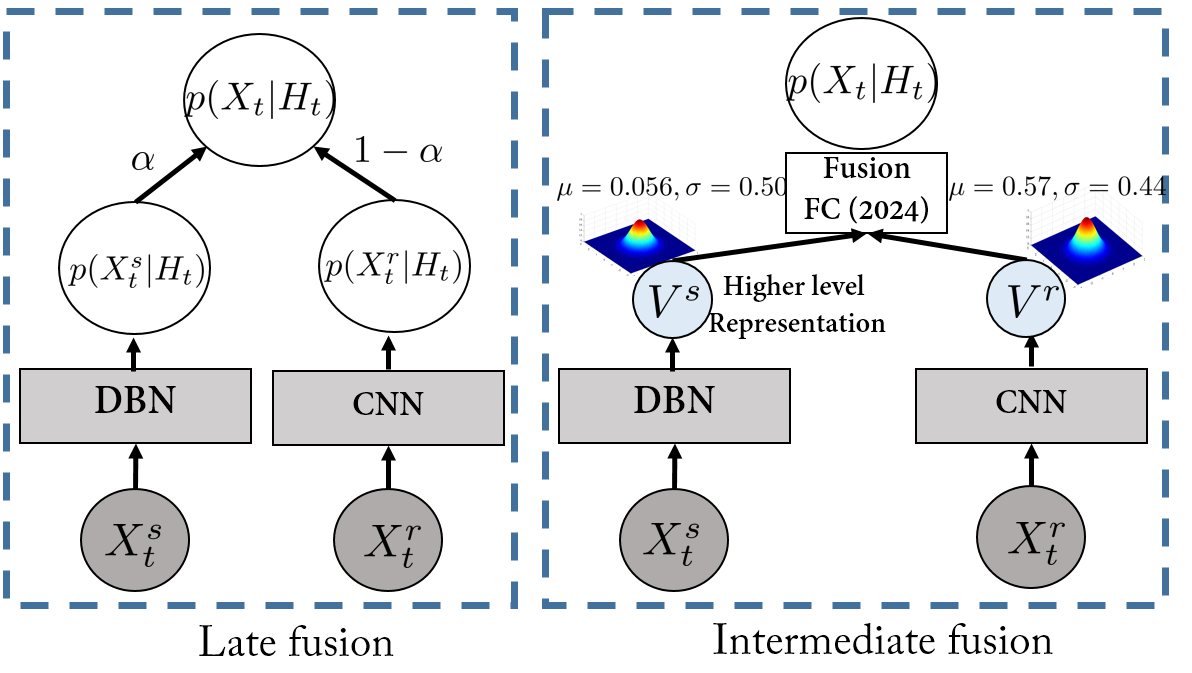
\includegraphics[width=0.5\textwidth]{images/Fusion_combined}
\vspace*{-2mm}
\caption{
\small{
Multimodal dynamic networks with late fusion scheme (left) and intermediate fusion scheme (right).
The late approach simply combines the emission probabilities from two modalities.
In the intermediate fusion scheme, each modality (skeleton and \RGBD) is first pre-trained separately,
and their high-level representation \highSK and \highRGBD (the penultimate node layers of their neural networks)
are concatenated to generate a shared representation. The two sub-modules in the resulting architecture are trained jointly.}
  }\label{fig:fusion}
\end{figure}



\endinput


%%%%%%%%%%%%%%%%%%%%%%%%%%%%%%%%%%%%%%%%%%%%%%%%%%%%%%%%%%%%%%%%%%%%%


\section{Experiments and Analysis}

This Section reports the experiments performed to validate our model.
First, we will introduce the ChaLearn dataset, and then present the experimental protocol we followed.
In Section~\ref{sec:results}, we will present and analyse the obtained results, including a discussion
on the modeling elements.
Finally, Section~\ref{sec:ComputationalComplexity} will briefly discuss the computational complexity of the approach.




\subsection{Chalearn LAP Dataset}
\label{sec:chalearn}

\begin{figure}[t]
        \centering
        \begin{subfigure}[c]{.5\textwidth}
        \centering
                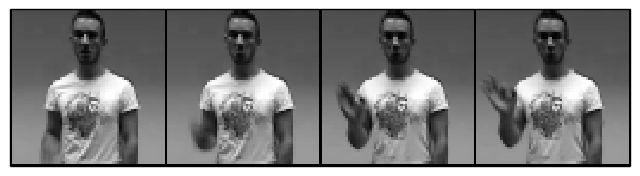
\includegraphics[width=8cm,height=2cm, clip]{images/3dcnn_filters/original_images_gray_body_ok}
                \caption{``OK"}
        \end{subfigure}%
        %
        \\
        \begin{subfigure}[c]{0.5\textwidth}
        \centering
                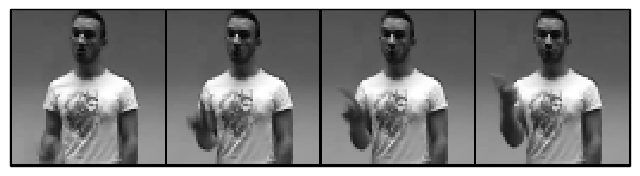
\includegraphics[width=8cm,height=2cm, clip]{images/3dcnn_filters/original_images_gray_body_ncnp}
                %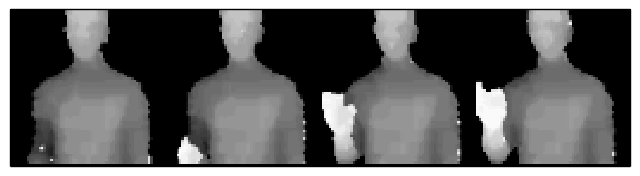
\includegraphics[width=2cm,height=3cm, trim=120 100 100 50, clip]{images/3dcnn_filters/original_images_depth_body_ok}
                \caption{``Non ce ne piu"}
        \end{subfigure}
        \\
       \begin{subfigure}[c]{0.5\textwidth}
        \centering
                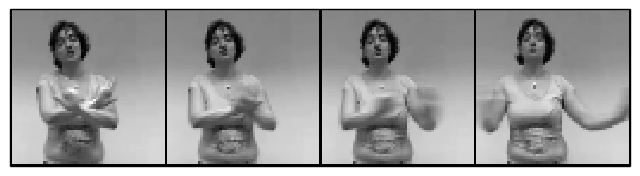
\includegraphics[width=8cm,height=2cm, clip]{images/3dcnn_filters/original_images_gray_body_basta}
                %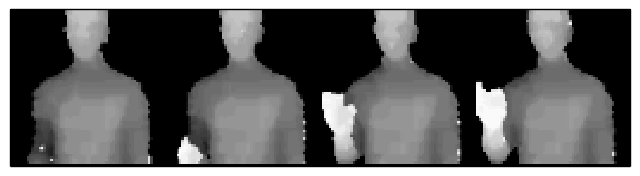
\includegraphics[width=2cm,height=3cm, trim=120 100 100 50, clip]{images/3dcnn_filters/original_images_depth_body_ok}
                \caption{``Basta"}
        \end{subfigure}
       \\
       \begin{subfigure}[c]{0.5\textwidth}
        \centering
                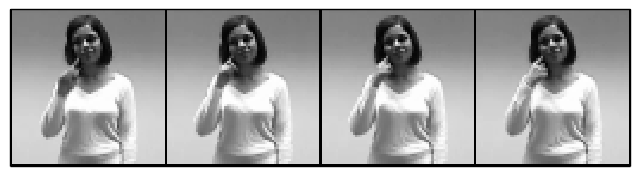
\includegraphics[width=8cm,height=2cm, clip]{images/3dcnn_filters/original_images_gray_body_buonissimo}
                %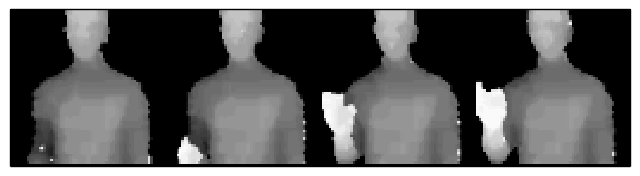
\includegraphics[width=2cm,height=3cm, trim=120 100 100 50, clip]{images/3dcnn_filters/original_images_depth_body_ok}
                \caption{``Buonissimo"}
        \end{subfigure}
               \\
       \begin{subfigure}[c]{0.5\textwidth}
        \centering
                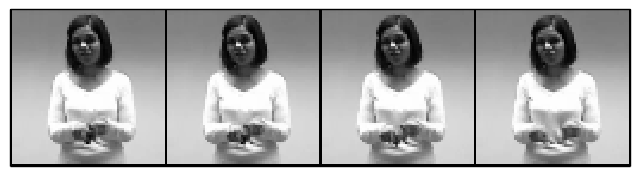
\includegraphics[width=8cm,height=2cm, clip]{images/3dcnn_filters/original_images_gray_body_daccordo}
                %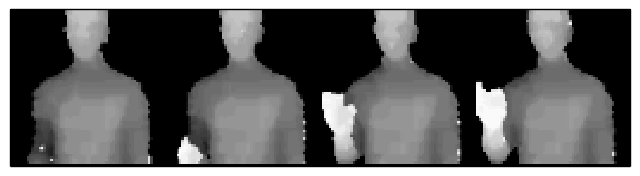
\includegraphics[width=2cm,height=3cm, trim=120 100 100 50, clip]{images/3dcnn_filters/original_images_depth_body_ok}
                \caption{``Daccordo"}
        \end{subfigure}
                       \\
       \begin{subfigure}[c]{0.5\textwidth}
        \centering
                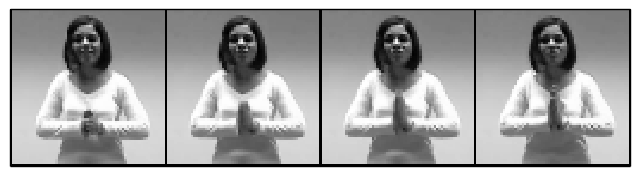
\includegraphics[width=8cm,height=2cm, clip]{images/3dcnn_filters/original_images_gray_body_combinato}
                %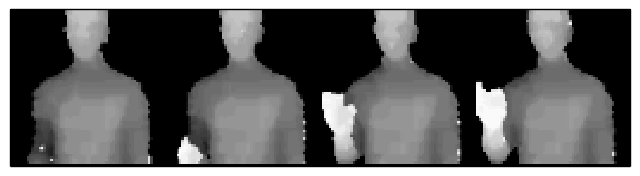
\includegraphics[width=2cm,height=3cm, trim=120 100 100 50, clip]{images/3dcnn_filters/original_images_depth_body_ok}
                \caption{``Combinato"}
        \end{subfigure}
  \caption{
\mycomline{Add other examples of gestures, interesting to comment upon take them from chalearn website.
From the confusion matrix, i would propose: ``Basta'', buenissimo, daccordo, combinato}
\dwucomline{We may not show all the examples here}
Examples of gestures in the Chalearn dataset.
Note that some gestures primarily differ primarily in hand pose but not the arm motions, like ``OK'' \emph{vs} ``Non ce ne piu''. ``Basta" and ``Combinato" are the gestures that got mostly misclassified.
  }
\label{fig:chalearnclasses}
\end{figure}




\mycomline{In this part, provide more information about the dataset: description, content, types of gestures (what are the classes), illustration of the gestures with some pictures (esp. for gestures that have impact on data -for example, expand fig 14 where yoou have the two ok and noncepiu examples with other ones, and put it earlier in the document. why is the dataset challenging ?\\
Also, provide some statistics about the dataset:
 rough duration of the gestures (average, min max). How many person are performing the gestures, how many occurrences per class, is the dataset balanced}

The dataset used in this work is provided by the ChaLearn LAP \cite{chalearnLAP} gesture spotting challenge\footnote{\href{http://gesture.chalearn.org/2014-looking-at-people-challenge/data-2014-challenge}{http://gesture.chalearn.org/2014-looking-at-people-challenge/data-2014-challenge}}.
%
The focus  is on ``multiple instance, user independent spotting" of gestures, which means learning to recognize gestures from several instances for each category performed by different users, drawn from a gesture vocabulary of 20 Italian cultural/anthropological signs.
A gesture vocabulary is a set of unique gestures, generally related to a particular task.

The challenge dataset contains 940 videos sequences, each performed by a single person and composed of 10 to 20 gesture instances for a total of around $14,000$ gestures.
%
There are 20 gesture classes, \emph{i.e.} \emph{vattene, vieniqui, perfetto, furbo, cheduepalle, chevuoi, daccordo, seipazzo, combinato, freganiente
    , ok, cosatifarei, basta, prendere, noncenepiu, fame, tantotempo, buonissimo, messidaccordo, sonostufo}, with a number a samples well balanced between classes.
% statistics of the gestures here:
The average length of gestures is 39 frames, the minimum frame number for a gesture is 16  and the maximum frame number is 104.

This dataset is challenging because the ``user independent" setting and some of gestures differ primarily in hand pose but not the overall arm motions as illustrated in Fig.~\ref{fig:chalearnclasses}

\mycomline{(to be presented/commented)}

In terms of data, three modalities are provided with the input videos: the sequence of skeleton joints, and the RGB and depth images
(including a segmentation of the person performing the gesture).
%For the input sequences, there are three modalities provided, \emph{i.e.} skeleton, RGB and depth images (with user segmentation).
% This dataset  is on ``multiple instance, user independent learning and continuous gesture spotting"~\cite{ICMI} of gestures.
% In the 3 track, there are more than 14,000 gestures.

 \begin{table}[t]
   \centering
        \begin{tabular}{|l|c|}\hline
            { Gesture }  &\makebox[5em]{ Length}\\\hline\hline
            {\small vattene }            &  38.0   \\\hline
            {\small vieniqui }           &  36.1   \\\hline
            {\small perfetto }           &  36.7  \\\hline
            {\small furbo }              &  40.1   \\\hline
            {\small cheduepalle }        &  36.9    \\\hline
            {\small chevuoi }            &  35.9    \\\hline
            {\small daccordo }           &  40.2   \\\hline
            {\small seipazzo }           &  43.5    \\\hline
            {\small combinato }          &  45.6    \\\hline
            {\small freganiente }        &  37.8    \\\hline
            %%%%%%%%%%%%%%%%%%%%%%%%%%%%%%%%%%%%%%%%%%
            {\small ok }                 &  30.8    \\\hline
            {\small cosatifarei }        &  41.9    \\\hline
            {\small basta }              &  35.7   \\\hline
            {\small prendere }           &  37.9    \\\hline
            {\small noncenepiu }         &  37.5    \\\hline
            {\small fame }               &  41.3    \\\hline
            {\small tantotempo }         &  39.1    \\\hline
            {\small buonissimo }         &  43.5   \\\hline
            {\small messidaccordo }      &  44.5    \\\hline
            {\small sonostufo }          &  39.9    \\\hline
        \end{tabular}
\vspace*{-2mm}
    \caption{\dwucomline{Average length of a gesture, this table won't be included in the final version, but just to show to JMO.}
          }
          \label{Table_score_fusion}
\end{table}


\subsection{Experimental protocol}

\subsubsection{Training and evaluation protocol}

We follow the ChaLearn experimental protocol, in which the input sequences are split into 700 videos for training, and 240 sequences for testing and reporting results.
Note that the   test sequences  are not segmented a priori and the gestures must be detected within a continuous data stream
which, in addition to the targeted gestures, also contains noisy and out-of-vocabulary gestures.
%
Furthermore, in the experiments, we split the training videos into 650 videos for learning the actual neural network model parameters, and 50 videos
used as validation data for monitoring the training performance or selecting hyper-parameters.


\subsubsection{Performance measures}

Several measures can be used to evaluate the gesture recognition performance.
%
In this work, we adopted the ChaLearn performance measure known as the Jaccard index, which relies on a frame-by-frame prediction accuracy.
More precisely, if $GT_i$ denotes the sequence of ground truth labels in video $i$, and $R_i$ the algorithm output, the Jaccard index
of the video is defined as:
\begin{align}
\jaccardindex_i(GT_i, R_i,g) = \frac{N_s(GT_i, R_i,g)}{N_u(GT_i, R_i,g)},
\\
\mbox{and } \jaccardindex_i = \frac{1}{|{\cal G}_i)|} \sum_{g \in {\cal G}_i} \jaccardindex_i(GT_i, R_i,g)
\end{align}

where $N_s(GT_i, R_i, g)$ denotes the number of frames where the ground truth and result agree on the gesture class $g$,
and $N_u(GT_i, R_i, g)$ denotes the number of frames labeled as a gesture frame $g$ by  either the ground truth or the algorithm,
and ${{\cal G}_i}$ denotes the set of gestures either in the ground truth or detected by the algorithm in sequence $i$\footnote{Note that 'non gesture'

frames are thus excluded from the counts.}. The average of the $\jaccardindex_i$ over all test videos is reported as performance measure.
%
Note that experimentally, this measure tends to favours having more false positives than missing true positives, in order to increase the numerator.
%Effective ways to detect false positives should be an interesting aspect of future work.

Being defined at the frame level, the Jaccard index can vary due to variations of the segmentation (both in the ground truth and recognition)
at gesture boundaries, which can be irrelevant from an application viewpoint.
%
Thus, we also defined performance at the gesture event level by following the commonly used PASCAL challenge intersection over union criterion.
More precisely, if for a gesture segment $G$, we have $\frac{G \cap R}{G \cup R} >  0.5$, where R denotes a recognized gesture
segment of the same class, then the  gesture is said to be recognized.
%
If the same relation holds but with a gesture segment of another class, the prediction is incorrect.
Otherwise the gesture is rated as undetected. This allows us to define the \eventaccuracy, \eventconfused and \eventmissed performance measures at the video level,
which are further averaged over test sequences for reporting.


\begin{figure*}[t]
        \centering
        \begin{subfigure}[c]{.8\textwidth}
                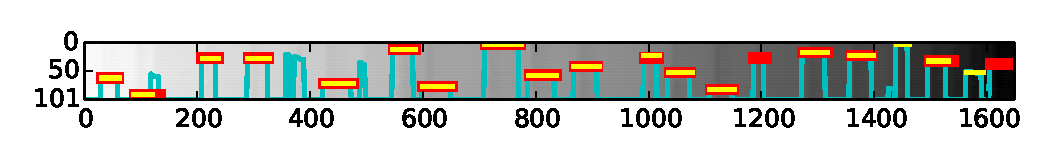
\includegraphics[width=\textwidth]{images/path/Sample0700_sk}
%\vspace*{-3mm}
                \caption{Viterbi decoding from skeleton input.}
                \label{Sample0700_sk}
        \end{subfigure}%
        ~ %add desired spacing between images, e. g. ~, \quad, \qquad, \hfill etc.
          %(or a blank line to force the subfigure onto a new line)

        \begin{subfigure}[c]{0.8\textwidth}
                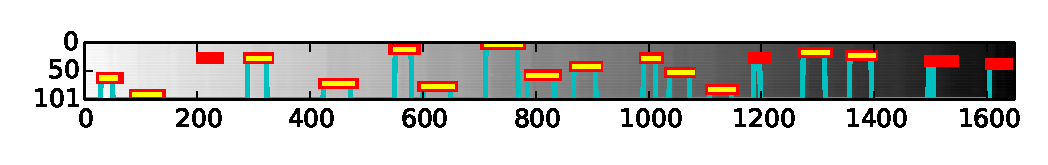
\includegraphics[width=\textwidth]{images/path/Sample0700_cnn}
%\vspace*{-3mm}
                \caption{Viterbi decoding from RGB-D input.}
                \label{Sample0700_cnn}
        \end{subfigure}

        ~ %add desired spacing between images, e. g. ~, \quad, \qquad, \hfill etc.
          %(or a blank line to force the subfigure onto a new line)
        \begin{subfigure}[c]{0.8\textwidth}
                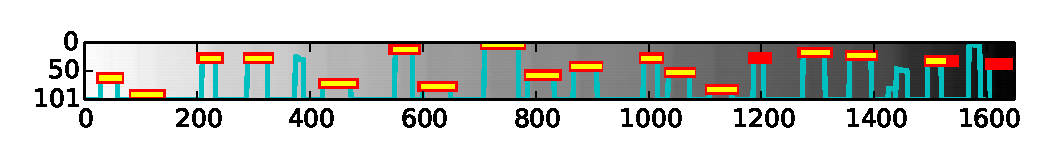
\includegraphics[width=\textwidth]{images/path/Sample0700_combined}
%\vspace*{-3mm}
                \caption{Viterbi decoding from the late fusion of skeleton and RGB-D input.}
                \label{Sample0700_combined}
        \end{subfigure}

  \caption{Viterbi decoding of sample sequence \#700, using skeleton (top), RGB-D (middle) and late fusion system (bottom). The x-axis represents the time and the y-axis represents the hidden states of all the classes and of the ergodic state at the state \emph{101}. Red lines are the ground truth labels, cyan lines represent the viterbi shortest path and yellow lines are the predicted labels. Two modules exhibit complementary behaviors and generally the skeletal module outperforms the depth module. The fusion exploits the complementary properties, \emph{e.g.} around frame 200 the skeleton help solving with the missed detection from the 3DCNN module, while around frame 1450, the 3DCNN module can help suppress the false positive prediction given by skeleton module.
  }\label{fig:Sample0700_comparison}
\end{figure*}

\subsubsection{Tested systems}

We evaluated the recognition performance made by the HMM applied to the emission probabilities estimated from either
the skeleton data, the RGBD image data, the late fusion scheme, and the early fusion scheme.
%
Note that in all cases the HMM output was further filtered to avoid false alarms,
by considering gesture segments of less than 20 frames as noise and discarding them.
%Note that in all cases the HMM output was further filtered as follows to avoid false alarms.
%First, predicted gesture segments of less than 20 frames were considered as noise and discarded.

%
%% \dwucomline{Actually during the actual test the threshold is set at -inf which does not serve as postprocessing}
%% In addition, longer but noisy gesture segments whose log-probability (including both emission and transition probabilities)  measured over the viterbi path
%% was lower than a threshold were discarded.
%% %
%% This threshold was set by optimizing the Jaccard index on the validation set  of the training data.


%%%%%%%%%%%%%%%%%%%%%%%%%%%%%%%%%%%%%%%%%%%%%%%%%%%%%%%%%%
 \begin{table}[t]
   \centering
        \begin{tabular}{|l||*{2}{c|}}\hline
            {Module }
            &\makebox[5em]{Validation}&\makebox[5em]{Test}
            \\\hline\hline
            {\small Skeleton -- DBDN }            &  0.783    & 0.779 \\\hline
            {\small RGBD -- 3DCNN }      &  0.752    & 0.717 \\\hline%\hline
            {\small Multimodal Late Fusion }              &  0.817    & 0.809 \\\hline
            {\small Multimodal Early Fusion }             &  0.800    & 0.798 \\\hline
        \end{tabular}
\vspace*{-2mm}
    \caption{Results in terms of Jaccard index \jaccardindex for the different network structures and modalities modeling the emission probabilities.
          }
          \label{Table_score_fusion}
          \label{tab:jaccardperformance}
\end{table}
%%%%%%%%%%%%%%%%%%%%%%%%%%%%%%%%%%%%%%%%%%%%%%%%%%%%%%%%%%


%%%%%%%%%%%%%%%%%%%%%%%%%%%%%%%%%%%%%%%%%%%%%%%%%%%%%%%%%%

 \begin{table}[rt]
   \centering
        \begin{tabular}{|ll||*{2}{c|}}\hline
            %\backslashbox{Module}{Evaluation Set}
             &  \% &  \makebox[5em]{Validation}&\makebox[5em]{Test}       \\\hline\hline
            \multirow{2}{*}{Skeleton - DBDN}       & \eventaccuracy                & 86.3     & 83.6 \\
                                            &  \eventconfused           & 11.4     & 12.3 \\
                                            &  \eventmissed           &  2.3     &   4.1 \\\hline\hline
            \multirow{2}{*}{RGB-D - 3DCNN}    & \eventaccuracy              & 78.7     & 75.8  \\
                                            &  \eventconfused           & 5.2     &  4.5 \\
                                            &  \eventmissed           & 16.1     & 19.7  \\\hline\hline
            \multirow{2}{*}{Multimodal Late Fusion}   &  \eventaccuracy    & 87.9     & 86.4 \\
                                                      &  \eventconfused    & 9.1     & 8.7 \\
                                                      &  \eventmissed      & 3.0      & 4.9 \\\hline
           \multirow{2}{*}{Multimodal Early Fusion}   &  \eventaccuracy    & 86.5     & 85.5\\
                                                      &  \eventconfused    & 7.3      & 6.8 \\
                                                      &  \eventmissed      & 6.2      & 7.7 \\\hline
        \end{tabular}
\vspace*{-2mm}
    \caption{
       Gesture classification performance at the event level, in percentage of the number of ground truth gestures.
%\mycomline{table to be finished as for the skeleton}
          }
          \label{tab:eventperformance}
\end{table}

%%%%%%%%%%%%%%%%%%%%%%%%%%%%%%%%%%%%%%%%%%%%%%%%%%%%%%%%%%

\subsection{Results}\label{sec:results}

\mycomline{Confusion matrices are fine. However, would it be possible to know the classifiction accuracy of the different classes, for each modality? (i.e the diagonal elements of the confusion matrix? i.e. for instance to look at lowest/highest results? and it improves with fusion?}

\mypartitle{Overall results.}
%
The overal performance of the algorithms are given in Tables~\ref{Table_score_fusion} and~\ref{tab:eventperformance}.
%
As can be observed from both performance measures, the skeleton module usually  performs better than the RGB-D module.
In addition, its generalization capability  is better than that of the RGB-D module,
especially when measured with the Jaccard index where there is almost no drop of performance between the validation and test data.
%
One possible explanation is that the information in the skeleton data is more robust, as it benefited from training using huge and highly
varied data~\cite{shotton2011real}: around on million images from both realistic and synthetic depth images were used to train
the decision forest classifiers involved in the joints extraction.
%
On the over hand, as the  RGBD module relies on  the raw data and was learned only from the ChaLearn training set, it may
suffer from some overfitting.
%
Another interesting conclusion that can be drawn from Table~\ref{tab:eventperformance} is that while most errors from the RGB-D module are due to under detection
(the \eventmissed rate is 19.7\%, whereas it is only 4.1\% for the skeleton), the skeleton module is more reactive to gesture activity, but makes more mistakes
(the \eventconfused rate is 12.3\% vs 4.5\% for RGB-D).


Finally, the results also demonstrate  that the combination of both modalities is more robust,
as shown by the recognition rate increase and the smaller drop in the generalization performance
%, both at the \jaccardindex and event level
(for instance the decrease of the \eventaccuracy rate is lower than for the skeleton data alone).



%%%%%%%%%%%%%%%%%%%%%%%%%%%%%%%%%%%%%%%%%%%%%%%%%%%%%%%%%%
\begin{figure}[t]
        \centering
        \begin{subfigure}[c]{.36\textwidth}
                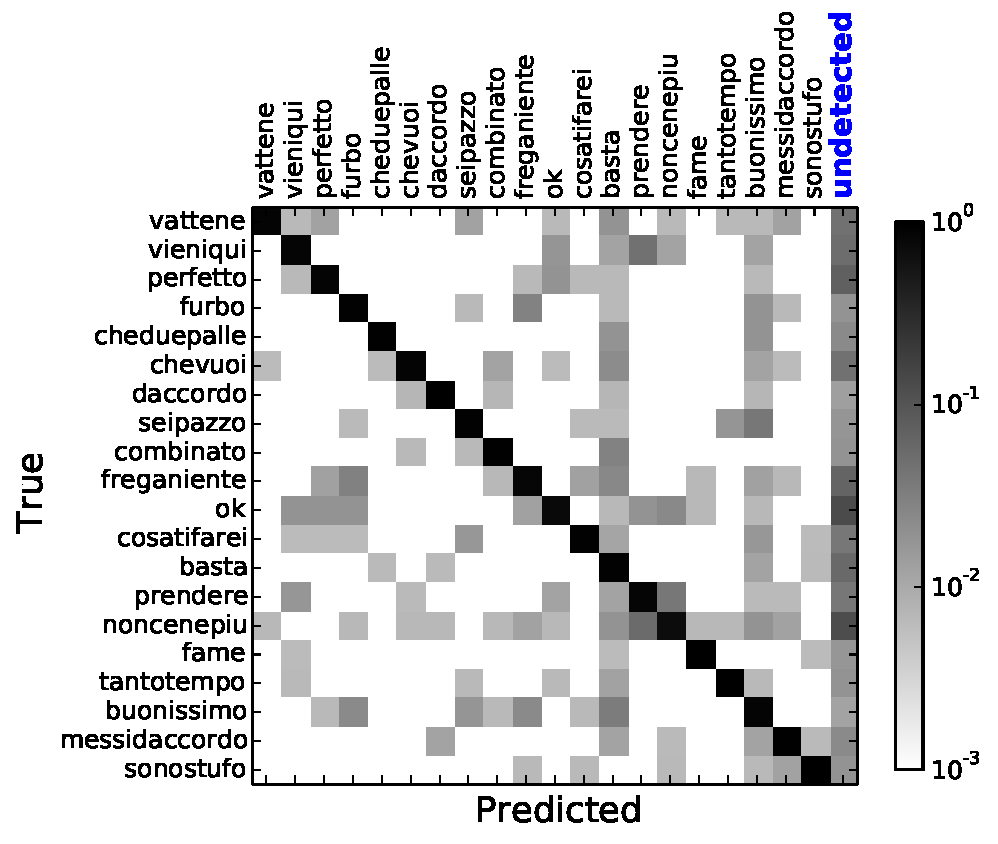
\includegraphics[width=\textwidth]{images/cm/cm_sk}
\vspace*{-3mm}
                \caption{Skeleton - DBDN}
                \label{sk_cm}
        \end{subfigure}%
        ~ %add desired spacing between images, e. g. ~, \quad, \qquad, \hfill etc.
          %(or a blank line to force the subfigure onto a new line)

        \begin{subfigure}[c]{0.36\textwidth}
                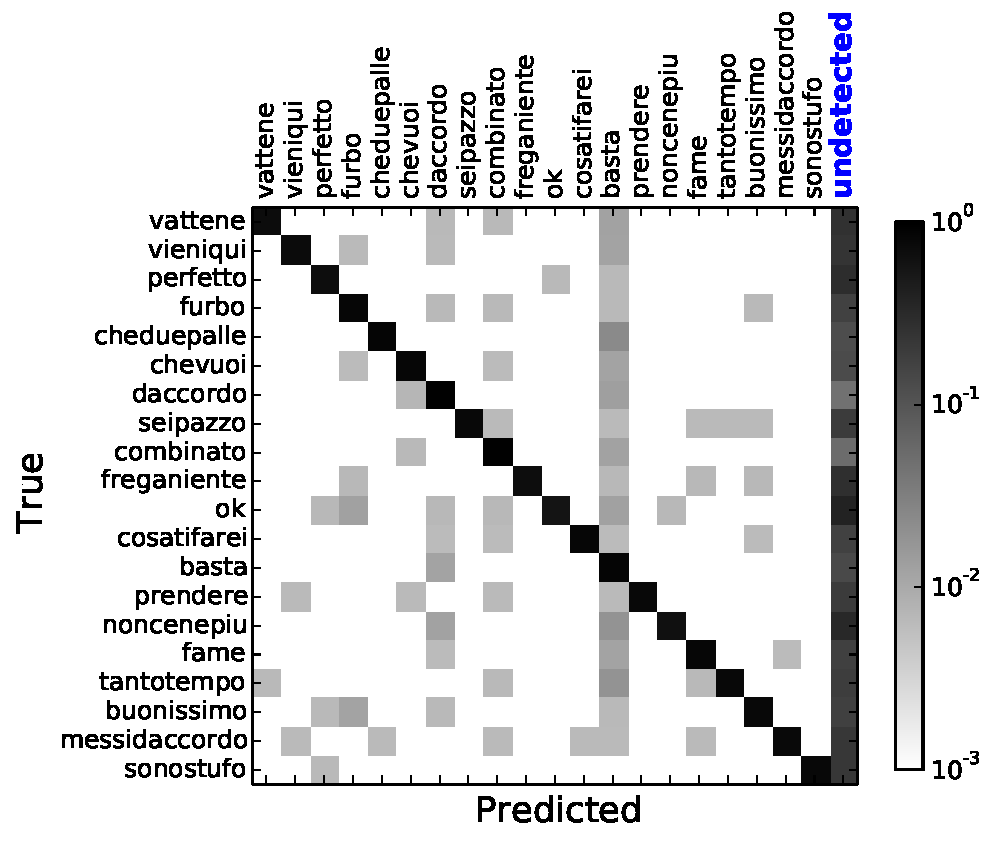
\includegraphics[width=\textwidth]{images/cm/cm_cnn}
\vspace*{-3mm}
                \caption{RGBD - 3DCNN}
                \label{cnn_cm}
        \end{subfigure}

        ~ %add desired spacing between images, e. g. ~, \quad, \qquad, \hfill etc.
          %(or a blank line to force the subfigure onto a new line)
        \begin{subfigure}[c]{0.36\textwidth}
                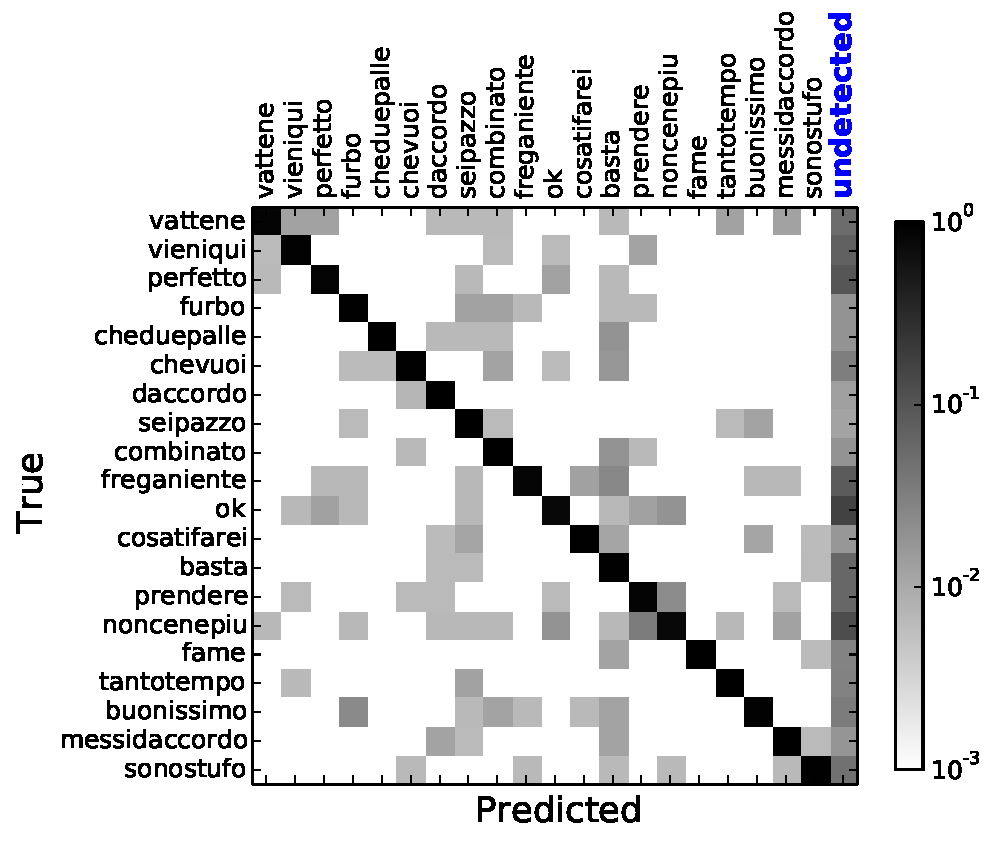
\includegraphics[width=\textwidth]{images/cm/cm_combination}
\vspace*{-3mm}
                \caption{Multimodal Late Fusion}
                \label{fusion_cm}
        \end{subfigure}

  \caption{Confusion Matrices  for the different modalities.}
\label{fig:confusion_matrix}
\end{figure}
%%%%%%%%%%%%%%%%%%%%%%%%%%%%%%%%%%%%%%%%%%%%%%%%%%%%%%%%%%

\mypartitle{Confusion matrices.}
%
The confusion matrices in Fig.~\ref{fig:confusion_matrix} better illustrate the complementarity of the behaviors of the two modalities.
%
The higher underdetection of RGB-D is clearly visible (whiter matrix, except last 'undetected' column).
%

We can also notice that some gestures are more easily recognized than others,
or catch the difficult instances of other gestures.
This is the case for instance of the ``Basta" gesture,
whose arms motion  resembles the  start and end of the arm motion of many other gesture (see Fig.~\ref{fig:chalearnclasses}).
Whatever the modality, it thus tends to be over-detected for all gesture classes, whenever the
likelihood of the instances are low when being evaluated using the HMM states associated with their true label
due to too much variability.
%
Similarly, the hand movement and pose of the ``Buenissimo" gesture is present in several other gesture classes,
whose instances are then often confused with ``Buenissimo" when relying on the skeleton information alone.
%
However, as these gestures differ primarily in their hand pose, such confusion is much more reduced using the RGB-D domain,
or when fusing  the skeleton and RGB-D modules.
%
The complementary properties of the two modalities is also illustrated from the Viterbi path decoding plot in Fig.~\ref{fig:Sample0700_comparison}.
In general, the benefit of this complementarity between arm pose/gesture and hand pose
can be observed from the whiter confusion matrix than in the skeleton case (less confusion due to hand pose information from RGB-D)
and much less under-detection than in the RGB-D case (better upper-body pose discrimination thanks to skeleton input).
%

However, the modalities by themselves have more difficulties to correct the recognition errors which are due to variations coming from the performer,
like differentiating  people that gesticulate more (see Fig.~\ref{fig:bodydynamics}).

\mypartitle{Late vs. Early fusion.}
%
The results in Table~\ref{tab:jaccardperformance} and~\ref{tab:eventperformance} show that the early fusion system 
improved individual modalities, but without outperform the late fusion system. 
%
The result is counter-intuitive, as we would have expected the cross-modality learning in the early fusion scheme 
to result in better emission probability predictions, as compared to the simple score fusion in the late system.
%
One possible explanation is that the independance assumption of the late scheme better preserves both
the complementarity and redundancy of the different modalities, properties which are important for fusion.
%
Another related explanation is that one individual modality may have a dominant effect in the early fusion learning process, 
thus skewing the network towards learning that specific module and lowering the importance of the other module outputs 
%
The mean activations of the neurons for each modules in Fig.~\ref{fig:fusion} indicate the aforementioned conjecture.
 The mean activation of skeleton module neurons is predominantly larger than the RGBD ConvNet's (0.57 \emph{vs.} 0.056). Though that skeleton module has logistic units whereas ConvNet module has relu unit~\cite{DBLP:journals/corr/PigouODHD15}, the mean activations of the two are not directly comparable. However, 10 times the difference of mean activation indicates the bias during the multimodal fine-tuning phase that could cause the less than expected performance.

\mycomline{In this comment on the results and benefit of the temporal model, as we discussed.}
%

\mypartitle{HMM benefit.}


\mypartitle{Comparison with the state-of-the-art. In particular, add discussion that other temporal module could be used,
including those that could lead to the training of a full deep-neural network.  }
%

To investigate the benefit of temporal modelling of the proposed system, we compare the model that discards temporal modelling. Specially, once, we collect the emission probability \emissionprob{}, we average the hidden states for each gesture class and obtain the frame based gesture class prediction \gestureEmissionProb where \gesturehiddenstateFrame denotes the gesture variables. After temporal smoothing for each frame, a threshold for cutting the begin and end of active gesture is chosen by a validation set.

\dwucomline{A new Fig. will be included}
The performance of recent state-of-the-art techniques is given in Table~\ref{tab:soa}.

\mycomline{Distinguish handcrafted features and neural net approaches. explain the differences in models that potentially lead to the difference.}


%%%%%%%%%%%%%%%%%%%%%%%%%%%%%%%%%%%%%%%%%%%%%%%%%%%%%%%%%%

\begin{figure}[tb]
        \centering

        \begin{subfigure}[c]{.2\textwidth}
        \centering
                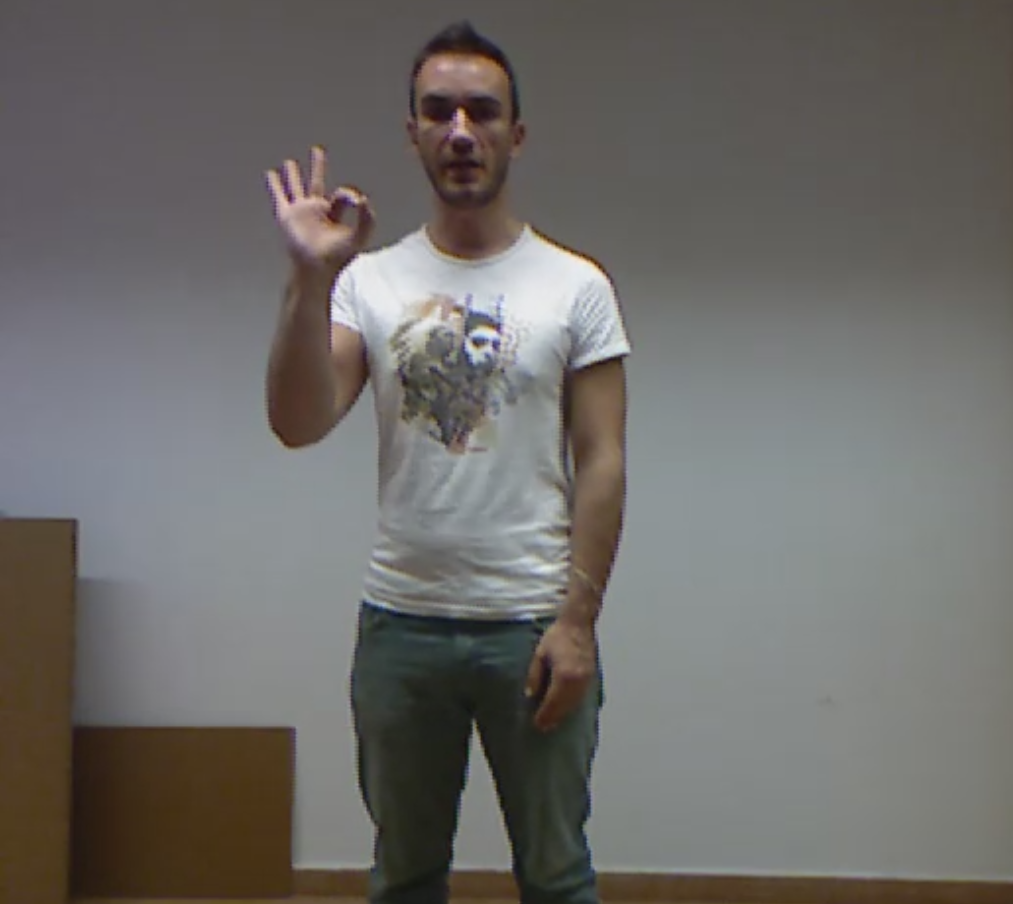
\includegraphics[width=3cm,height=3cm, trim=120 100 100 50, clip]{images/good}
      \vspace*{-2mm}
                \caption{Well-recognised}
        \end{subfigure}%
        %
        \begin{subfigure}[c]{0.2\textwidth}
        \centering
                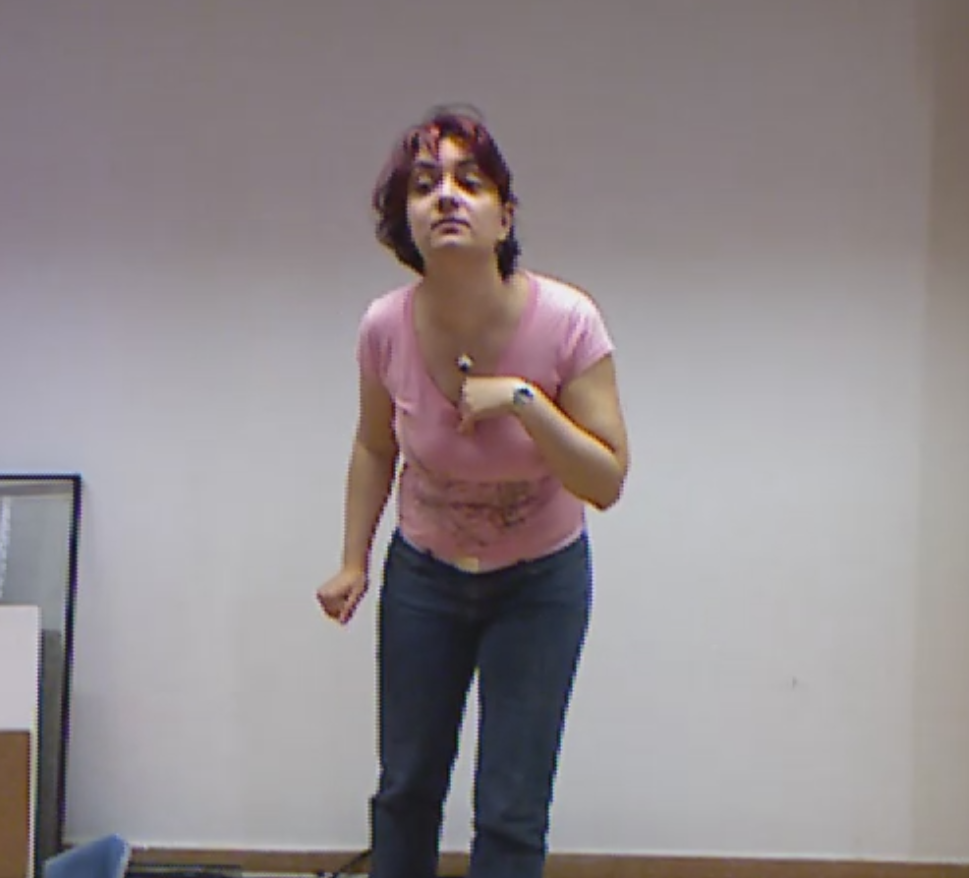
\includegraphics[width=3cm,height=3cm, trim=120 100 100 50, clip]{images/bad}
      \vspace*{-2mm}
                \caption{Poorly-recognised}
        \end{subfigure}
      \vspace*{-3mm}
  \caption{
\mycomline{Show more sample to illustrate the dynamic - would be good to show the instances for the same gestures - the jaccard index below are obtained using which module?}
Examples of performer variations in the  upper body dynamic.
While most performers tend to keep their upper-body static while performing the gesture leading to good recognition performance (left, Jaccard index of 0.94),
others vehemently move their body when doing the gestures, making them harder to recognize (right, Jaccard index of 0.34).
}
\label{fig:bodydynamics}
\end{figure}



%%%%%%%%%%%%%%%%%%%%%%%%%%%%%%%%%%%%%%%%%%%%%%%%%%%%%%%%%%%%
 \begin{table}[t]
   \centering
        \begin{tabular}{|l||*{3}{c|}}\hline
            {Module}
            &\makebox[3em]{Skeleton}&\makebox[6em]{RGBD}&\makebox[3em]{Fusion}
            \\\hline\hline
            {~\cite{neverova2014multi}} Deep Learning (Step 4)                  &   0.7891     &  0.7990      & \textbf{0.8449}\\\hline
            {~\cite{neverova2014multi}} Deep Learning (multiscal)               &   0.8080     &  0.8096      & \textbf{ 0.8488}\\\hline
            {~\cite{Monnier2014multi}} 3 Set Skeletal \& HOG                   &   0.791     & -           & 0.8220 \\\hline
            {~\cite{Chang2014multi}}   Handcrafted features                       &  \textbf{0.7948}     & -           & 0.8268\\\hline
            {~\cite{Peng2014multi}}    Dense Trajectory                         &  -          & \textbf{0.7919}      & -\\\hline
            {~\cite{lio2014deep}}      CNN                                      &  -          & 0.7888      & -\\\hline
            {~\cite{wu2014deep}}    Deep Learning                               &  0.7468     & 0.6371      & 0.8045\\\hline \hline
            \textbf{\emph{DDNN}} (this work)                                    &  0.7792    & 0.7168  & 0.8091\\\hline
        \end{tabular}
    \caption{
\mycomline{Add one or two worse results; separate hand crafted features from neural net methods.}
    Comparison of results in terms of the ChaLearn Jaccard index with state-of-the-art related works.
          }
          \label{tab:soa}
\end{table}


\subsection{Computational Complexity}
\label{sec:ComputationalComplexity}

We can distinguish between two complexity: the training one, and the test one.

\mycomline{Say a few words about the training complexity (which part takes longer -skeleton ? RGBD? - and how long does it take on the Chalearn dataset.}

\mypartitle{Complexity at training time.}
Although training the deep neural network using stochastic gradient descent is computationally intensive, the reuse of our pre-train network parameters could help with the better initialisation of the fusion network and fast convergence. Different modality training time also varies. Specifically, the training time of each epoch for DBN skeleton module is less than 300 seconds and allowing training 500 epochs within 2 days. The training time of each epoch for 3DCNN of RGB-D  module is much computational expensive, taking more than 10,000 seconds. Hence, 40 epochs takes around 5 days to train. The fusion network's parameters are initialised with individual modules

\mypartitle{Complexity at test time.}
%
Given the learned models,  our framework can perform real-time video sequence labelling with a low inference cost.
%
More specifically, a single feed forward neural network incurs linear computational time ($\mathcal{O}(T)$),
and is efficient because it requires only matrix products and convolution operations.
The complexity of the Viterbi algorithm is itself of $\mathcal{O} (T* |S|^2)$, where
$T$ is the number of frames and $|S|$ the number of states, and thus performs real-timegiven our state-space.

In practice, using a modern GPU (GeForece GTX TITAN Black), our multimodal neural network can be deployed at 90 FPS using the
Theano library~\cite{Bastien-Theano-2012}.
The preprocessing part takes most of the time and our un-optimized version runs at 25 FPS, while the
 Viterbi decoding  runs at 90 FPS. Hence, the overall system can achieve faster than real-time performance.





\endinput



\section{Conclusion and future work}
\label{sec:conclusion}

Hand-engineered, task-specific features are often task-specific and time-consuming to design. % Less adaptive than what? I changed this because there is no direct comparison
This difficulty is even more pronounced with multimodal data as we would like the features
to relate to multiple data sources.
%
In this paper, we presented a novel deep dynamic neural network (DDNN)
%that relied on  deep belief networks
%and 3D convolutional neural networks
for learning contextual frame-level representations and modelling emission probabilities in the framework of an HMM temporal model.
%
Different feature learning methods (DBN and 3DCNN) suited to the heterogeneous inputs from skeletal joints, RGB images, and depth images
were proposed, as well as different fusion schemes.
%
Experimental results on bi-modal gesture time series  show that the multimodal DDNN framework can learn
good models of the joint space of multiple sensory inputs, improving over  unimodal input.



There are several directions for future work.
%
Our results with those of other recent works suggest that learning features directly from data is a very important research direction
and that with more and more data and flops-free  computational power, learning-based methods are not only more generalisable to many domains,
but also are powerful in combination  with other well-studied probabilistic graphical models
for dynamical modelling and reasoning.
%
In this view, the learning of  better shared and complementary representation among multimodal  and heterogeneous  inputs,
as done in~\cite{neverova2014moddrop}, requires more exploration.
%
In addition, while the proposed HMM provided a good basis for the temporal modeling of gestures,
other more discriminant temporal approaches such as Conditional Random Field or further and better variants
\cite{wang2006hidden} could be directly exploited at their advantage in conjuction with our deep neural network  learning approach.
%
Ultimately, in a logical way, these two research directions converge into the investigation of
a single and unified deep learning framework fusing heterogeneous modalities
by using recent Recurrent Neural Networks such as Long Short Term Memory~\cite{graves2009novel} for modelling the temporal component of the problem.

%\mycomline{I would cite papers providing neural temporal models, rather than the one already applied to the gesture task}
%such as the work of ~\cite{DBLP:journals/corr/PigouODHD15}.

\endinput

%%%%%%%%%%%%%%%%%%%%%%%%%%%%%%%%%%%%%%%%%%%%%%%%%%%%%%%%%%%%%%%%%%%%%
\appendices
% you can choose not to have a title for an appendix
% if you want by leaving the argument blank
\section{Details of the Code}
The python code using for this work can be found at: \\
\footnotesize{\verb+https://github.com/stevenwudi/chalearn2014_wudi_lio+}


% use section* for acknowledgment
\ifCLASSOPTIONcompsoc
  % The Computer Society usually uses the plural form
  \section*{Acknowledgments}
\else
  % regular IEEE prefers the singular form
  \section*{Acknowledgment}
\fi

The authors would like to thank Sander Dieleman for his guidance in building, training and initialising convolutional neural networks.


\bibliographystyle{IEEEtran}
\bibliography{tPAMI2015}

\newpage

\newpage

\newcommand{\rev}[1]{{\noindent {\bf Comment:} {\it #1}}~\\}
\newcommand{\ans}[1]{{\noindent {\bf Response:} #1}~\\}
\newcommand{\td}[1]{{\noindent {\bf TODO:} #1}~\\}




\newcommand{\PM}[1]{
~\\
``\ldots{\em #1}\ldots''
}


% -----------------------------------------------------------------------------------
% -----------------------------------------------------------------------------------
\newpage
{\LARGE \noindent Response to Associate Editor}\newline



\rev{Reviews of the paper have been received. In general comments are positive. Still one reviewer suggests some interesting extra analyses of the proposed method. Please carefully address all reviewers comments for a second review round of the paper. Please provide your revision by July 31th.}

\ans{We would  like to thank the associate editor's general positive comments on our paper. We also would like to thank reviewers' careful and insightful suggestions for improving the paper. Following are some common points that were mentioned by the reviewers and we list the most notable changes below. The point to point responses are provided afterwards.

\begin{itemize}
\item In the previous version for multimodal fusion, we used the late fusion scheme  $s = a * s1 + (1-a)*s2$ where $a$ is chosen by cross-validation. In this revision, we implement an early fusion scheme in Section~\ref{early_fusion} that a new-top level perceptron layer is created to combine two models' output as in Fig.~\ref{early_fusion_fig}. The new multimodal neural network's parameters are initialised by the previously trained individual module, taking advantage of different modules� intrinsic properties and making the network converge much faster. The early fusion system uses pre-trained weights. The results are reported in  Section~\ref{early_fusion} and Table~\ref{Table_score_fusion}.

\item The Related Works section has been moved after the Introduction section. We also follow reviewers' suggestions and include discussions of related works concerning works of: 1) exploiting temporal models in the context of gesture recognition; 2) literature for RGBD data using deep learning -
    ``Wang \emph{et al.}~\cite{wang2006hidden} introduced a discriminative hidden-state approach for the recognition of human gestures. However, their discriminative training is limited for pre-segmented gesture sequences and one layer of hidden states might not learn powerful enough high level representations for a larger corpus."
    ``In the field of deep learning from RGBD data, Socher \emph{et al.}~\cite{socher2012convolutional} proposed a single convolutional neural net layer for each modality as input to multiple, fixed-tree RNNs in order to compose higher order features for 3D object classification. The single convolutional neural net layer provides useful translational invariance of low level features such as edges and allows parts of an object to be deformable to some extent. The pooled filter responses are then given to a recursive neural network to learn compositional features and part interactions.
    Gupta \emph{et al.}~\cite{gupta2014learning} proposed a geocentric embedding for depth images that encodes height above ground and angle with gravity for each pixel in addition to the horizontal disparity. The depth image was represented by three channels: horizontal disparity, height above ground and angle with gravity. This augmented representation allows the CNN to learn strong features than by using disparity (or depth) alone. "

\item Experimental analysis. We have included some time analysis in Section~\ref{Computational Complexity} and visualisation of response maps after learnt filters in Fig~\ref{3dcnn_filters}.

\item Explanation of intuition behind higher level presentation of the skeleton features. We include Section \ref{Deep Dynamic Neural Networks} to explain the intuition behind higher level representation for skeleton joint features which appeared in our previous CVPR paper but was not included in the previous submission. We think this part is one of major contributions of the paper and inclusion of this section makes the journal paper more self-contained.
\end{itemize}
}

% -----------------------------------------------------------------------------------
\newpage
{\LARGE \noindent Response to Reviewer 1}\newline

We thank the reviewer for his time and comments and positive appreciation of the paper.
Below, we provide our answers to his comments and to the unclear points that were raised, 
and what we have done to clarify the paper and take comments into account. 
Note that in our answer, all references (Equations, Figures) 
refer to the new version unless stated otherwise. 


\rev{The article is easy to read and well structured. The methodology is not strictly novel but its application in the gesture domain with the multimodal fusion makes the article worth reading. Although results are arguably a little behind the maximum performance ones the overall impression of the article is favorable and I believe the community may benefit to check the ideas included in this paper.

The article proposes a framework for dynamic data augmenting a HMM with deep learning techniques and apply this to gesture segmentation and recognition. Gestures segmentation and recognition is a difficult problem. The article tackles this difficulty by means of pure data driven approaches similar to the ones used for speech recognition. The particularities of the computer vision domain are handled accordingly.}

\ans{Thank you for your review and positive outlook of the paper. We are also aware that our results are arguably a little behind the maximum performance, and this may be due to the network initialisation and multimodal neural network learning. We have included extra experimental analysis and early fusion implementation to further extend the broadness of the paper.}

% -----------------------------------------------------------------------------------
\newpage

{\LARGE \noindent Response to Reviewer 2}\newline

We thank the reviewer for his time and comments.
Note that the article has been reworked significantly to better introduce and enhance the modeling elements.
% 
Below, we provide our specific answers to his comments and to the unclear points that were raised, 
and what we have done to clarify the paper and take comments into account.
%
Note that in our answer, all references (Equations, Figures) 
refer to the new version unless stated otherwise. 

\vspace{5mm}

\rev{In general, the manuscript is well written and is easy to follow. In the given case, it would be preferable to have the "Related work" section right after the introduction, as otherwise paper's contributions are not completely clear. Furthermore, there is certainly a vast literature on exploiting HMMs in the context of gesture recognition (as well as other temporal models, such as recurrent neural networks), which should be briefly summarized, the differences with the proposed solution should be highlighted.}

\ans{
Thank you for your comments and the recognition of easy readability of the paper. We have moved the related work section after the introduction section. Moreover, we have included the discussions of literature that utilise temporal models, e.g.,``Wang \emph{et al.}~\cite{wang2006hidden} introduced a discriminative hidden-state approach for the recognition of human gestures. However, their discriminative training is limited for pre-segmented gesture sequences and one layer of hidden states might not learn powerful enough high level representations for a larger corpus",  ``~\cite{socher2012convolutional} proposed a single convolutional neural net layer for each modality as input to multiple, fixed-tree RNNs in order to compose higher order features for 3D object classification."
}

\hfill

\textbf{\emph{Comments:}}
\emph{Authors claim to learn a model in the joint multi-modal space is a slight overstatement, as neural networks processing different modalities are trained completely independently with following averaging of produced scores.}

\textbf{Response:}
Thank you for your comments. In this revision, we implement the early fusion scheme in Section~\ref{early_fusion} that ``we adopt another layer of perceptron for cross modality learning taking the input from each individual net's penultimate layer.
The parameters of two neural networks (for skeleton and depth) are loaded from the previously trained individual module...The results for the early fusion system are reported in Tab.~\ref{Table_score_fusion}. The fusion network is initialised by the pre-trained model and stacked with one hidden layer with 2024 hidden unites. We fine-tune the network and stop the training when the validation error rate stops decreasing ($\sim$15 epochs)...However, we can see from Tab.~\ref{Table_score_fusion} that the early fusion system does not outperform the late fusion system. The result is counter-intuitive because we expect that the early fusion  multimodal feature learning would extract semantically meaningful shared representations, outperforming individual modalities, and the early fusion scheme�s efficacy against the traditional method of late fusion~\cite{wu2014multimodal}. One possible explanation could be that one individual module has dominant effect on the learning process so as to screw the network towards learning that specific module. The mean activations of the neurons for each module in Fig.~\ref{early_fusion_fig} indicate the aforementioned conjecture."

\hfill

\textbf{\emph{Comments:}}
\emph{State of the art in the experimental section should be mentioned more consistently. For fair comparison, first three lines in Table 3 should be:
[39] Deep learning (step 4): skeleton 0.7891, video 0.7990, fusion 0.8449 [39] Deep learning (multiscale): skeleton 0.8080, video 0.8096, fusion 0.8488 [40] 3 sets of skeletal features and HoG: skeleton 0.791, fusion 0.8220
Therefore, it shows that both learning-based and feature extraction-based approaches outperform the proposed method on each modality, as well as on a combination of them.
Furthermore, it would be interesting to see how the HMM contributes in the performance in comparison with simple voting based on frame-based predictions.}

\textbf{Response:}
Thank you for your detailed comments. We have amended the results table accordingly. The less than maximum performance could be due to the less than ideal settings and initialisations of the neural network. Nonetheless, we would like to argue that one major contribution of the paper is using the learning method for feature extraction and the utilisation of HMM for simultaneous gesture segmentation and recognition. We also present some brief analysis of why the fusion network didn't achieve expected performance gain and hope the experimental analysis could cast some light on the future research directions of the related problems.

\hfill

\textbf{\emph{Comments:}}
\emph{Visualization of the filter banks (section 3.3.4) in its current state is unnecessary as it does not provide any interesting insights on the interpretation of the learned features. Instead, the poorly formed filters rather indicate undertraining, or lack of training data given the model complexity, or suboptimality of training procedure.}

\textbf{Response:} We  include the response maps after filtering for both body and hand parts. We observe some interesting properties from the visualisation of the filter banks as in~\cite{socher2012convolutional} that ``Depth images have sharper edges and generally are smoother than the grayscale filters, though the distinctions are less obvious compared with the body versus hand filters."




\hrulefill

\subsubsection{Reviewer3}
\emph{Recommendation: Author Should Prepare A Minor Revision}

\textbf{\emph{Comments:}}

\emph{In general, I would be more excited if shared representations were learned from the skeleton and the RGB data, as done in multimodal deep learning. This is left for future work.  On the positive side, the CNN and DBN are technically sound and the results from their fusion are interesting.}

\emph{One would expect that the journal version of the paper would be more self-contained and easier to follow than the conference versions, but here I observe the opposite trend. For example, the older conference version ~\cite{diwucvpr14} explains the intuition behind the higher level representation of the skeleton features, but the journal version does not. The conference paper explains how the coordinate frames are built for the features, while this paper skips this part. The conference paper explains the datasets and visualizes the Viterbi paths better.}

\textbf{Response:} Thank you for your careful and positive review. We agree that in this journal version of the paper, some self-contained information has been omitted from the conference paper. In this revision, we have included more details. Specifically, 1) we include the Problem formation in Sec~\ref{Problem formation} that explains the intuition behind the higher level representation and the advantages offered by feed forward neural over GMMs. 2) we include another section for learning the higher level representation for skeleton joints features in Section~\ref{skeleon_high_level} from a pre-training point of view. The pre-training step is of crucial importance in learning the right initialisation of the deep belief networks using the sigmoid activation function.


\hfill

\textbf{\emph{Comments:}}
\emph{Section 2 does not help much the reader understand the formulation. For example:
 "At each time step, we have one observed random variable $X_t$: explain what these variables represent early (raw skeletan input / RGBD)  we have an unobserved variable $H_t$: describe at a high level the information that the unobserved variables capture, mention examples}

\textbf{Response:}
We have included the interpretation part as follows: ``A continuous-observation HMM with discrete hidden states is adopted for modelling higher level temporal relationships. At each time step $t$, we have one observed random variable $X_t$ which can be the skeleton input or depth/RGB input.
 The unobserved variable $H_t$ taking on values in a finite set  $\mathcal{H}=(\bigcup _{a \in \mathcal{A}} \mathcal{H}_a)$, where $\mathcal{H}_a$ is a set of states associated with an individual gesture $\textbf{\emph{a}}$ by force-alignment. The unobserved variable $H_t$ can be interpreted as a segment of an action $\textbf{\emph{a}}$. For example, for action sequence ``tennis serving", the action sequence can be dissected into $\mathcal{H}_{a_1}, \mathcal{H}_{a_2}, \mathcal{H}_{a_3}$ as: 1) raising one arm, 2) raising the racket, and 3) hitting the ball."



\hfill

\textbf{\emph{Comments:}}
\emph{The related work section is out of place after the technical sections and before the experiments.}

\textbf{Response:} We have moved the related work section after the introduction section.


\hfill

\textbf{\emph{Comments:}}
\emph{There is no point writing a loop for m=1:2 in Algorithm 1 and 2.}

\textbf{Response:} We have rewritten Algorithms 1 and 2 and merge the algorithms into a more succinct format.

\hfill

\textbf{\emph{Comments:}}
\emph{"the number of states ... is chosen as 5": any intuition here?}

\textbf{Response:} Thank you for the comment and this is a very good observation. The number of hidden states chosen uniformly as 5 in the paper might not be the optimal way of setting the number of hidden states for each gesture. We also experimented segmenting gestures into 10 states and obtained similar results. We reduce the hidden states from 10 to 5 in order to reduce the number of predicting classes and avoiding overfitting. The interpretation of choosing the number of hidden states for Markove Model is similar to choosing the number of hidden states for neural networks: it's more heuristically based. Ideally, we could set the number of hidden states according to the average length of the gesture sequence. But due to time constraint, we didn't train such neural networks.

\hfill

\textbf{\emph{Comments:}}
\emph{"10 frames are assigned to hidden state ...": why 10?}

\textbf{Response:} Thank you for the careful observation. This is actually a written error due to different number of hidden states used for our experiments. We rewrote the section as:
``\textbf{\emph{Hidden states} ($\mathcal{H}_a$): } Force alignment is used to extract the hidden states, \emph{i.e.} if a gesture token is 100 frames, the first $20= \frac{100}{5(N_{\mathcal{H}_a} )}$ frames are assigned to hidden state $\textbf{\emph{1}}$, the following 20 frames are assigned to hidden state $\textbf{\emph{2}}$, and so forth."



\hfill

\textbf{\emph{Comments:}}
\emph{it is hard to interpret the learned features on Figure 8. There is no intuition what the depth filters capture.}

\textbf{Response:} Because our filter size is $5\times5$ (smaller filter sizes tend to generalize better, ~\cite{simonyan2014very} used $3\times3$ convolution filters), it will be hard to interpret. However, we observe the similar effect as in paper~\cite{socher2012convolutional} for depth image filters and we include the following analysis:
``Visualisation of the $5\times5$ filters in the first layer for the different input channels . Interestingly, we observe the same effect as~\cite{socher2012convolutional} that the resulting filters from depth images have sharper edges which arise due to the strong discontinuities at object boundaries. While the depth channel is often quite noisy, most of the features are still smooth."

\hfill

%\textbf{\emph{Comments:}}
%\emph{ "multiple channel fusion outperforms individual modules by a large margin.": the difference is rather small based on the experiments}
%
%\textbf{Response:}


\hfill

\textbf{\emph{Comments:}}
\emph{Citations that could be added in the context of deep learning from RGBD data: "Convolutional-Recursive Deep Learning for 3D Object Classification", Socher et al., NIPS 2012}

\textbf{Response:}
Thank you for the suggested citation. And we now include in the related works section as follows:``In the field of deep learning from RGBD data, Socher \emph{et al.}~\cite{socher2012convolutional} proposed a single convolutional neural net layer for each modality as input to multiple, fixed-tree RNNs in order to compose higher order features for 3D object classification. The single convolutional neural net layer provides useful translational invariance of low level features such as edges and allows parts of an object to be deformable to some extent. The pooled filter responses are then given to a recursive neural network to learn compositional features and part interactions."

We also observe the same CNN filters as the paper that ``one interesting result is that depth channel edges are much sharper. This is due to the large discontinuities between object boundaries and background. While the depth channel is often quite noisy, most of the features are still smooth".

\hfill

\textbf{\emph{Comments:}}
\emph{"Learning Rich Features from RGB-D Images for Object Detection and Segmentation", Gupta et al., ECCV 2014}

\textbf{Response:}
We find the works in Gupta \emph{et al.}~\cite{gupta2014learning} interesting in a sense that CNN does not necessarily need to be trained from the raw images, and some handcrafted features may better help the network to learn more meaningful, higher level representations. And we have included this related work as follows.
``Gupta \emph{et al.} proposed a geocentric embedding for depth images that encodes height above ground and angle with gravity for each pixel in addition to the horizontal disparity. The depth image was represented by three channels: horizontal disparity, height above ground and angle with gravity. This augmented representation allows the CNN to learn strong features than by using disparity (or depth) alone."

\hfill

\textbf{\emph{Comments:}}
\emph{Another related work is the "Multimodal Deep Learning" by Ngiam et al., ICML 11. I would also like to see some discussion wrt "Hidden Conditional Random Fields for Gesture Recognition", Wang et al, CVPR 2006}

\textbf{Response:}
Thank you for suggesting very relevant works. We came across both papers. "Multimodal Deep Learning" essentially is the prototype for an early fusion model. Wang \emph{et al.}~\cite{wang2006hidden}) observed that one hidden layer is limited for learning a larger class corpus. Feature learning for skeleton modules is an essential part of this paper and we believe a higher level representation is more beneficial for gesture classification. Moreover, the partition function of CRF makes the discriminative training more difficult to train.  The similarity in the aforementioned paper with our proposed method is that both methods used a hidden layer for learning higher level representations. Recent advancement in feature learning and pre-training for DBN renders our proposed method more meaningful. We have included the following in the related works section:
``Wang \emph{et al.}~\cite{wang2006hidden} introduced a discriminative hidden-state approach for the recognition of human gestures. However, their discriminative training is limited for pre-segmented gesture sequences and one layer of hidden states might not learn powerful enough high level representation for a larger corpus."

\hfill

\hrulefill
\subsubsection{Reviewer4}
\emph{Recommendation: Author Should Prepare A Major Revision For A Second Review}

\textbf{\emph{Comments:}}
\emph{Late fusion: my greatest technical concern is that two deep models are trained and then combined with a weighted average: s = a * s1 + (1-a)*s2 where a is chosen by cross-validation. Instead, the authors could combine the two models by creating a new top-level perceptron layer which takes the two models as input. Then this whole structure could be trained jointly with back-propagation. I'd expect results to be (1)at least as good and (2) more philosophically unified. }

\textbf{Response:} We agree with your insightful observation and continue experimenting with the early fusion scheme in this revision. Our previous paper~\cite{wu2014multimodal} utilized the early fusion scheme for audio and skeleton modules for action recognition. We followed that strategy and perform the early fusion scheme using penultimate layer in Section\ref{early_fusion}.
``However, we can see from Table~\ref{Table_score_fusion} that the early fusion system does not outperform the late fusion system. The result is counter-intuitive because we expect that the early fusion  multimodal feature learning would extract semantically meaningful shared representations, outperforming individual modalities, and the early fusion scheme�s efficacy against the traditional method of late fusion~\cite{wu2014multimodal}. One possible explanation could be that one individual module has the dominant effect on the learning process so as to screw the network towards learning that specific module. The mean activations of the neurons for each modules in Fig.~\ref{early_fusion_fig} indicate the aforementioned conjecture."

\hfill

\textbf{\emph{Comments:}}
\emph{The analysis is a bit brief. More experiments and ablative analysis could be added. Specifically, can we interpret the failure patterns of the proposed model(s) and prior work? It would be interesting to see statements like [40] fails more often on gestures of X kind because HOG erases Y useful information or [39] does worse for Z because it handles time at an earlier stage of the pipeline. Then, also giving some qualitative examples of these failures.}

\textbf{Response:}
We agree that there is a lack of experiments� analysis, especially the failure patterns and lessons learnt from the experiments. We have included more analysis in the Experiment and Analysis section as follows:
``Examples of overall upper body movements� influence on the system performance. Left (score: 0.94) performer almost kept a static upper body whilst performing Italian sign language. Right (score: 0.34) performer moved vehemently when performing the gestures.\ref{good_bad_differ}"


\hfill

\textbf{\emph{Comments:}}
\emph{These extra experiments (considering joint training of a combined emission probability model) and qualitative interpretation could significantly affect the paper. Overall, the research is solid but needs significantly more work before publication.
RCNN: Last, it is entirely possible to train a recurrent neural network to perform Viterbi decoding. This may be difficult (requiring more training data) but would make the entire paper fit into a the deep learning framework. I cannot hold this against the authors, but some discussion might help.}

\textbf{Response:}
We have included more qualitative interpretation of the results.
We agree that a recurrent neural network could potentially replace the Viterbi decoding part to make the system as a more unified end-to-end system. This, however, may be left to the future work.


\hfill

\textbf{\emph{Comments:}}
\emph{
They use a 3d convolutional network. While the introduction makes it sound like this is for multiple-channels (e.g. RGB + Depth), sec. 3.3.2 makes it clear the 3rd dimension is time as the model processes 4 frame sub-sequences. I think, Fig. 6 could be clearer.}

\textbf{Response:}
Thank you for your detailed observation. Yes, the 3rd dimension of the input network is indeed the time axis. However, RGB and Depth data are treated as the two channels during the input phase. We detailed the description of the Figure as follows.
``The 3rd dimension of the input is time with 4 frames stacked together. The depth and RGB data are stacked (concatenated) together at Input. Hand and body part outputs are concatenated at H7."


\hfill

\textbf{\emph{Comments:}}
\emph{
Using RGB-D with deep learning is a common idea, explored by many concurrent works e.g. [A,B,C].
[A] Dosovitskiy, A., Springenberg, J. T., Riedmiller, M., \& Brox, T. (2014). Discriminative Unsupervised Feature Learning with Convolutional Neural Networks. arXiv Preprint arXiv: 1�13.
\newline
[B] Gupta, S., Girshick, R., Arbel�ez, P., \& Malik, J. (2014). Learning Rich Features from RGB-D Images for Object Detection and Segmentation. arXiv Preprint arXiv:1407.5736, 1�16. doi:10.1007978-3-319-10584-0-23
\newline
[C] Socher, R., Huval, B., Bhat, B., Manning, C. D., \& Ng, A. Y. (2012). Convolutional-Recursive Deep Learning for 3D Object Classification. Advances in Neural Information Processing Systems}

\textbf{Response:}
Thank you for suggesting related works.  We find the works in Gupta \emph{et al.}~\cite{gupta2014learning} interesting in a sense that CNN does not necessarily need to train from the raw images, and some handcrafted features may better help the network to learn more meaningful, higher level representations.
We have included the papers using deep learning for RBG-D data with discussions in the related works section:
``Gupta \emph{et al.} proposed a geocentric embedding for depth images that encodes height above ground and angle with gravity for each pixel in addition to the horizontal disparity. The depth image was represented by three channels: horizontal disparity, height above ground and angle with gravity. This augmented representation allows the CNN to learn strong features than by using disparity (or depth) alone."
``In the field of deep learning from RGBD data, Socher \emph{et al.} proposed a single convolutional neural net layer for each modality as input to multiple, fixed-tree RNNs in order to compose higher order features for 3D object classification. The single convolutional neural net layer provides useful translational invariance of low level features such as edges and allows parts of an object to be deformable to some extent. The pooled filter responses are then given to a recursive neural network to learn compositional features and part interactions."




\endinput



\end{document}
